
\subsection{Evaluación MOEA/D + EOP3 con ZDT3}

De igual manera a lo presentado para EOP1 y EOP2 vamos a realizar algunas pruebas para comprobar la efectividad del algoritmo con EOP3. Tanto utilizando una capacidad de cómputo de $10000$ evaluaciones como una de $4000$ evaluaciones (con los mismos repartos ya presentados).\\

\justify
\subsubsection{Experimentación con 1OOOO ev.}

En la \hyperref[fig:18]{\textit{figura 18}} presentamos tres gráficos pertenecientes a una ejecución característica del algoritmo con el operador evolutivo EOP3, $N=100, G=100$ y $T=15$ (para todos los casos se ha tomado un $15\%$  (recuérdese que en los anexos se muestran varias ejecuciones que validan las discusiones) el primer diagrama muestra el desarrollo de las soluciones en el espacio de objetivos a lo largo de la ejecución del algoritmo (en las distintas generaciones). En él podemos apreciar que, tal como esperábamos a medida que el algoritmo avanza (pasan las generaciones) las soluciones tinden a ir convergiendo hacia el frente real de Pareto (señalado en gris), de forma muy rápida. Otro aspecto a destacar es la diversidad, en los algoritmos evolutivos es corriente que las soluciones tiendan a concentrarse (se pierde diversidad); en este caso podemos ver dicha tendencia claramente, lo que produce lógicamente, que las soluciones no se distribuyan uniformemente, dándose un fénomeno habitual en algoritmos genéticos (del que hemos heredado este tercer operador) conocido como convergencia temprana (efecto indeseable).\\

En el segundo diagrama se presenta el conjunto de las soluciones no dominadas calculadas por el algoritmo, que parece estar bastante próximo al frente real de Paretoen cuanto a convergencia, pero sí es notable la pérdida clara de uniformidad en las soluciones frente a los resultados presentados en los operadores anteriores.\\

Finalmente, presentamos una gráfica comparativa para nuestro algoritmo y para el algoritmo \textit{NSGA-II}. Para ello hemos representado las soluciones en el espacio de objetivos, las cuales corresponden a la última generación de ejecuciones en iguales condiciones $(G=100, N=100)$ para ambos algoritmos. Podemos ver que en cuanto a convergencia (proximidad al frente real) el frente del nuestro algoritmo es ligeramente mejor que el frente proporcionado por  \textit{NSGA-II} (una mayoría de los puntos rojos están por debajo de los azules), mientras que en dispersión claramente los puntos del frente de \textit{NSGA-II} se distribuyen más uniformemente que los de nuestro algoritmo.\\

Veámos ahora unas gráficas análogas a las presentadas pero para el caso $(G=250, N=40)$ en la \hyperref[fig:19]{\textit{figura 19}} podemos notar que el comportamiento es similar al caso anterior dándose exactamente el mismo efecto, pero en este caso la diferencia con\textit{NSGAII} en convergencia es menor, debido a que NSGAII ha mejorado en ese aspecto (beneficiándose mucho más de las iteraciones que nuestro algoritmo, al que no le aportan mucho, a partir de un valor razonable). Si miramos el frente de soluciones no dominadas, vemos una situación muy similar a la anterior donde la mayoría de los puntos estan situados sobre el frente pero las soluciones no están uniformemente repartidas sino que tienden a estar bastante concentradas. En comparación con \textit{NSGAII} la convergencia de nuestro algoritmo parece ligeramente mejor mientras que en la distribución es sensiblemente peor.\\

Y en último lugar comprobemos cuál es el resultado de elevar el número de subproblemas frente al número de generaciones. Dado que según hemos visto hasta ahora lo convergencia suele ser rápida, y que el número de subproblemas favorecerá la diversidad, a priori el comportamiento debería ser satisfactorio. Veámos qué ocurre para el caso $(G=250, N=40)$ en las gráficas presentadas en la \hyperref[fig:20]{\textit{figura 20}}. Podemos notar que la convergencia es bastante buena pero la concentración de las soluciones y la rápida pérdida de la diversidad es patente. De hecho, si observamos el diagrama de las soluciones no dominadas podemos seguir notando que la distribución no es para nada uniforme. Si comparamos con la ejecución del \textit{NSGA-II} en este caso nuestro algoritmo es claramente mejor en convergencia y pero no en cobertura, aunque una mayoría de los puntos (lo veremos cuando analicemos las métricas) sí parecen estar dominados por los de nuestro algoritmo. \\

\begin{minipage}[H]{\linewidth}
\begin{minipage}[b]{0.3\linewidth}

\begin{figure}[H]
        \centering
        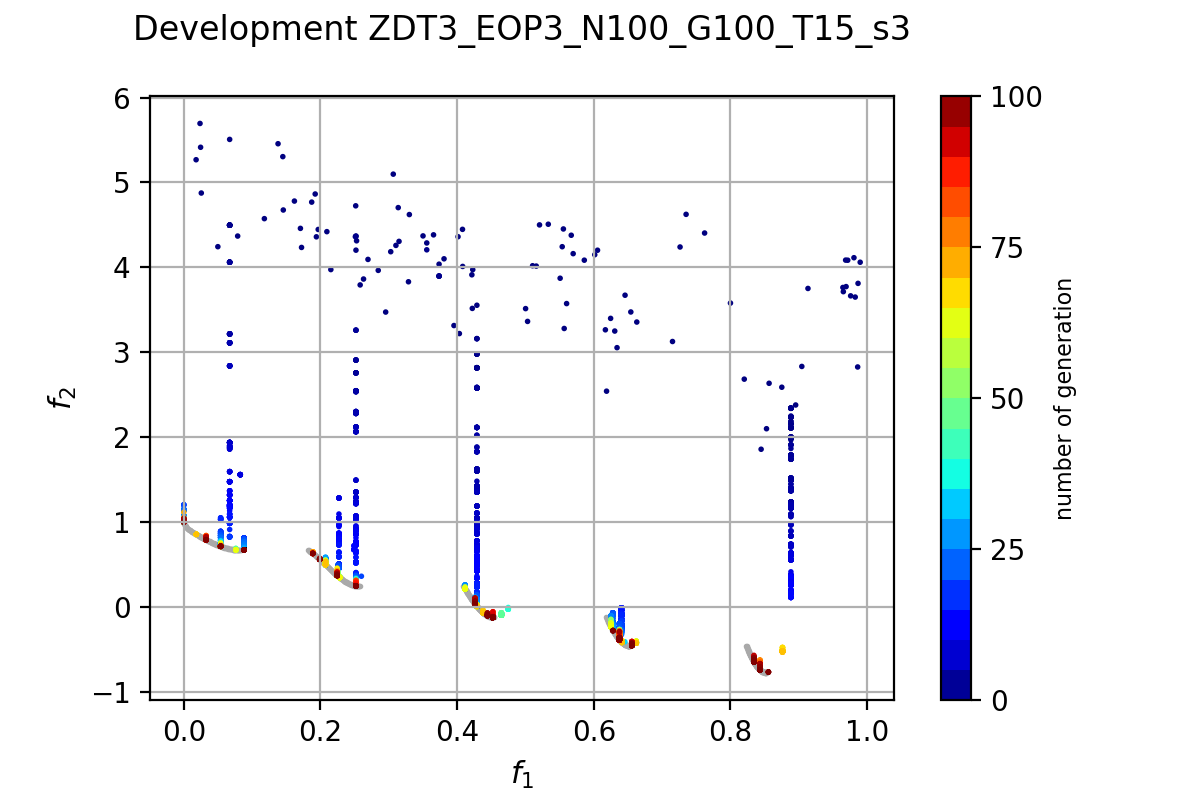
\includegraphics[scale=0.4]{figures/ZDT3_EOP3_N100_G100_T15/s3_dev.png}\\
        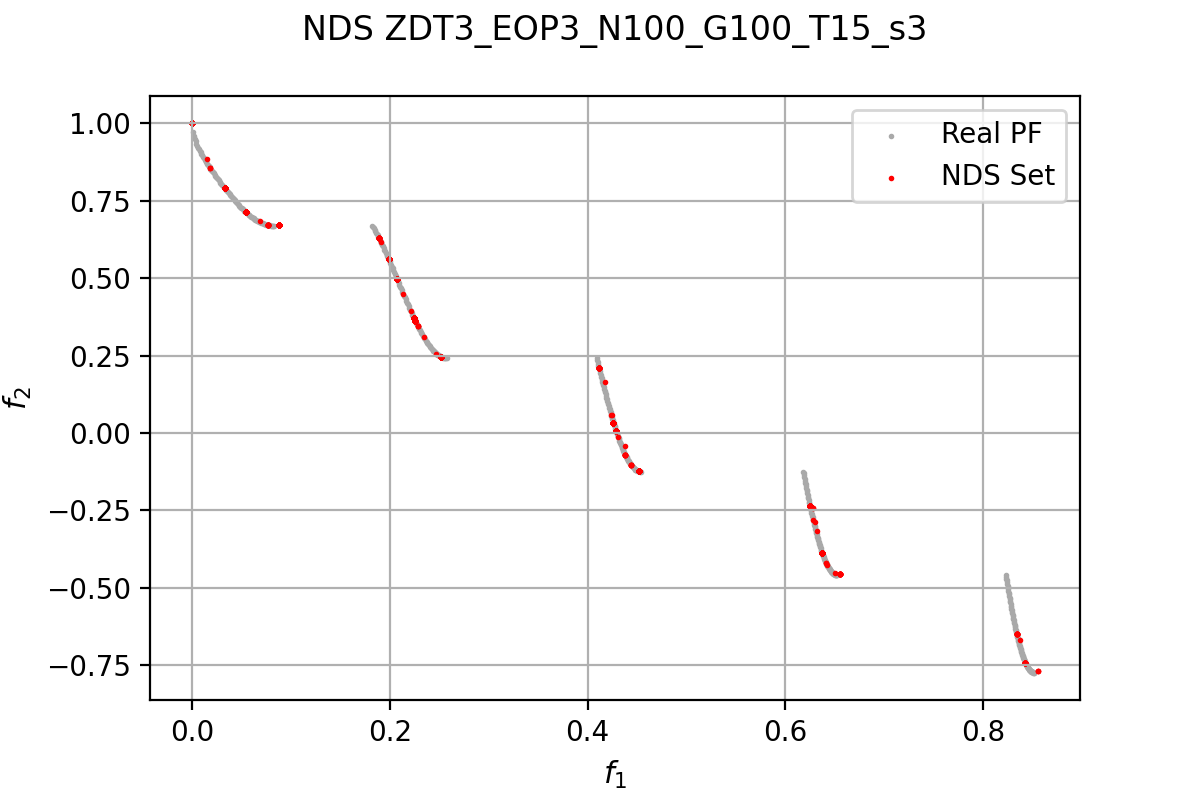
\includegraphics[scale=0.36]{figures/ZDT3_EOP3_N100_G100_T15/s3_nds.png}\\
        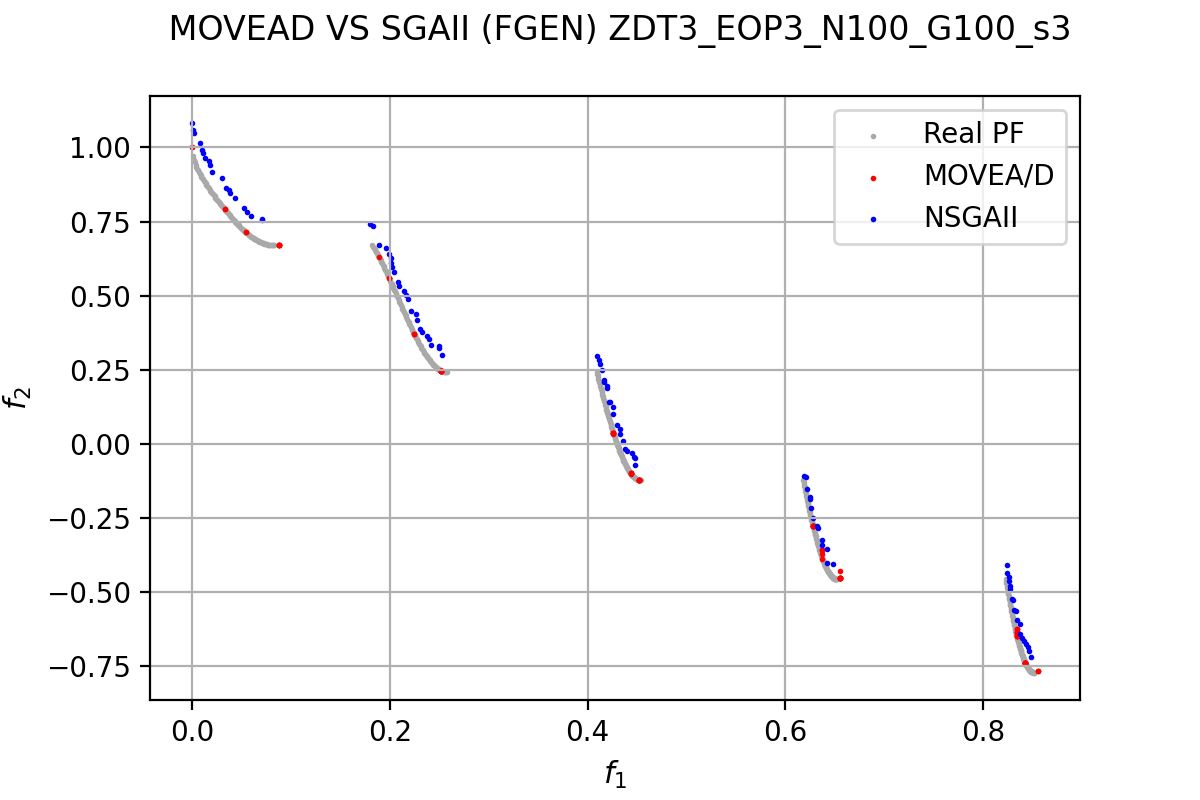
\includegraphics[scale=0.36]{figures/ZDT3_EOP3_N100_G100_T15/s3_comp.png}\\
        \caption{\centering MOEA/D + EOP3 (N100G100)}
        \label{fig:18}
    \end{figure}
\end{minipage} \quad
\begin{minipage}[b]{0.3\linewidth}
\begin{figure}[H]
        \centering
        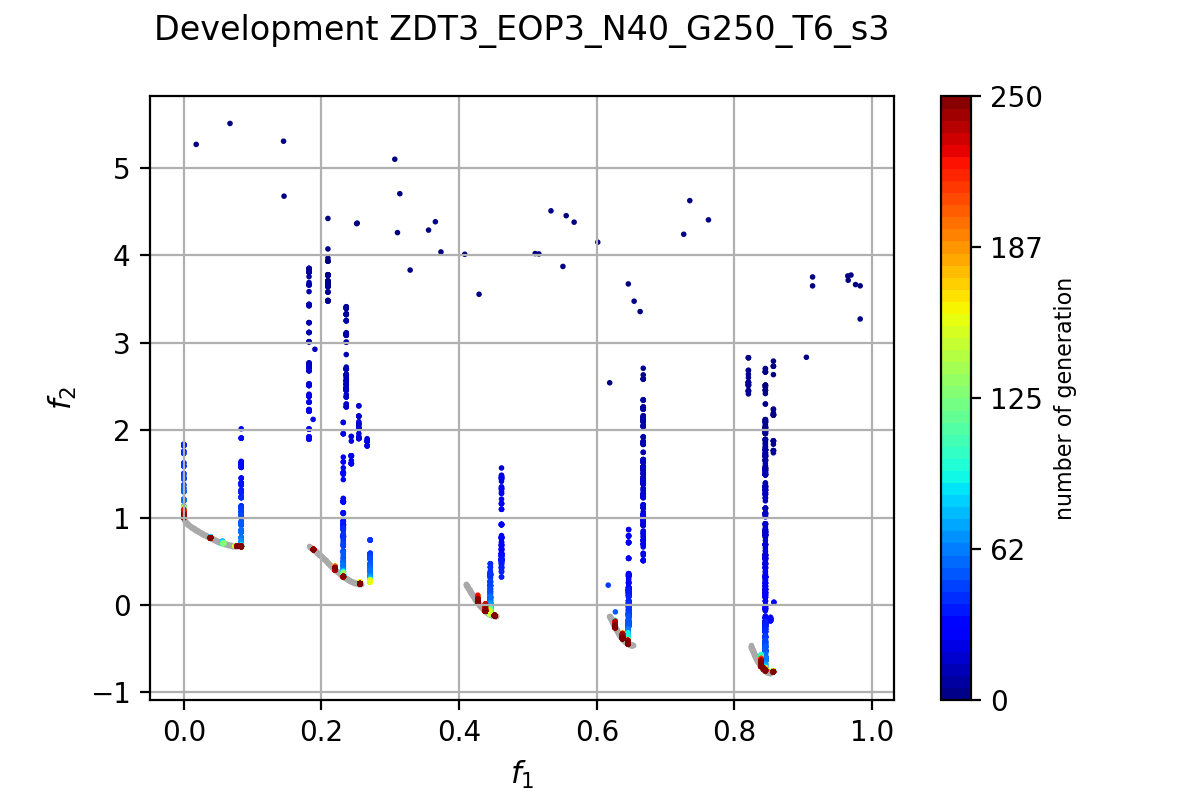
\includegraphics[scale=0.4]{figures/ZDT3_EOP3_N40_G250_T6/s3_dev.png}\\
        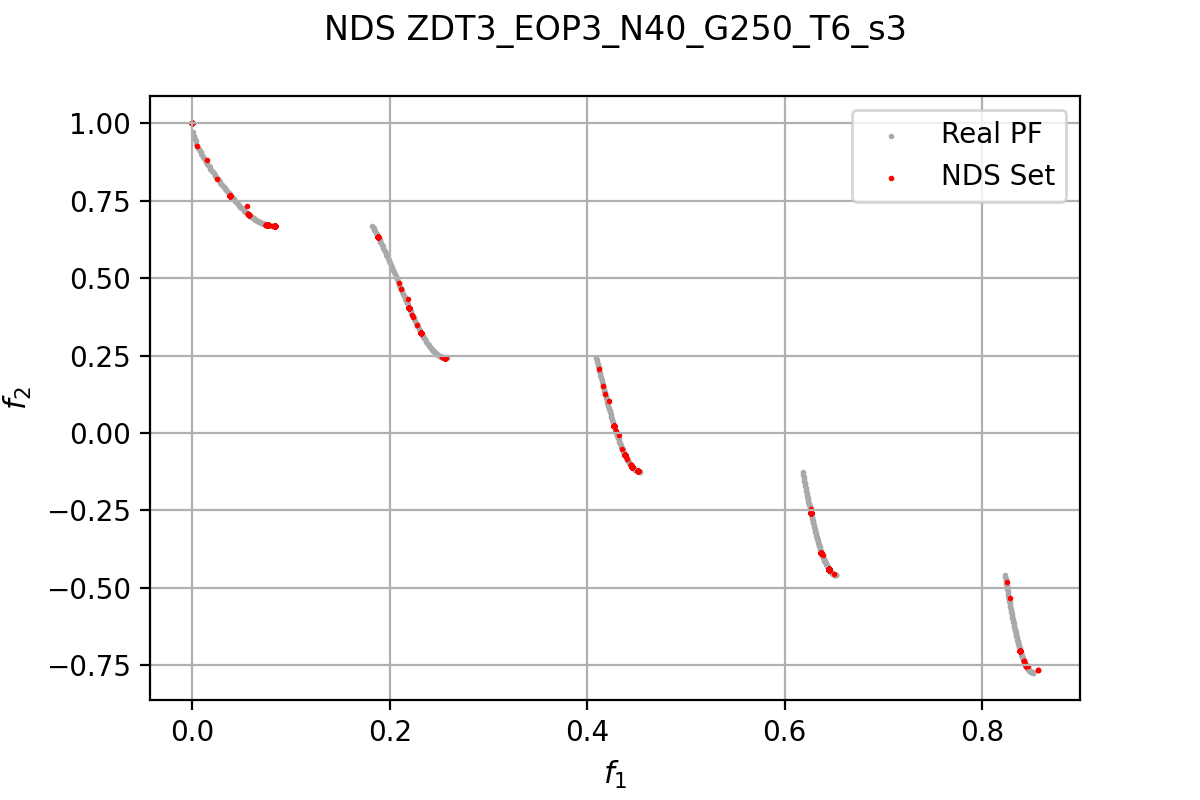
\includegraphics[scale=0.36]{figures/ZDT3_EOP3_N40_G250_T6/s3_nds.png}\\
        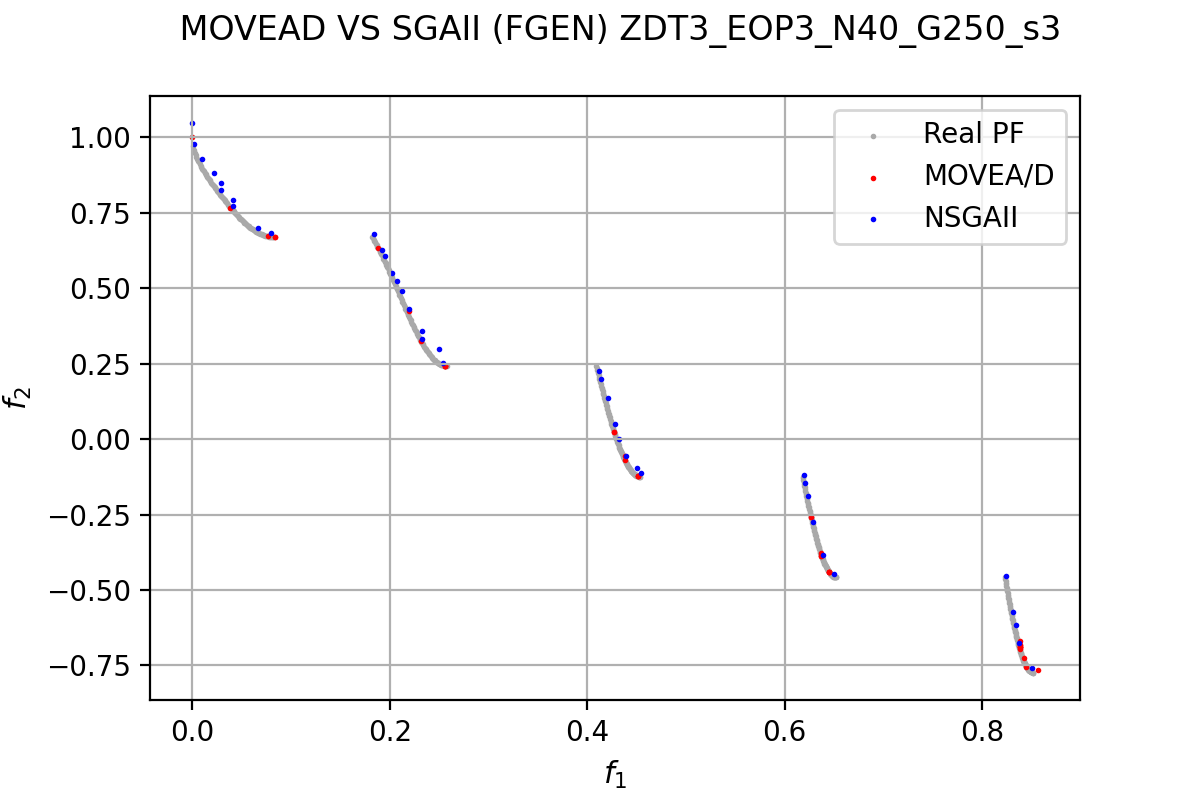
\includegraphics[scale=0.36]{figures/ZDT3_EOP3_N40_G250_T6/s3_comp.png}\\
        \caption{\centering MOEA/D + EOP3 (N40G250)}
        \label{fig:19}
    \end{figure}
\end{minipage} \quad
\begin{minipage}[b]{0.3\linewidth}
    \begin{figure}[H]
        \centering
        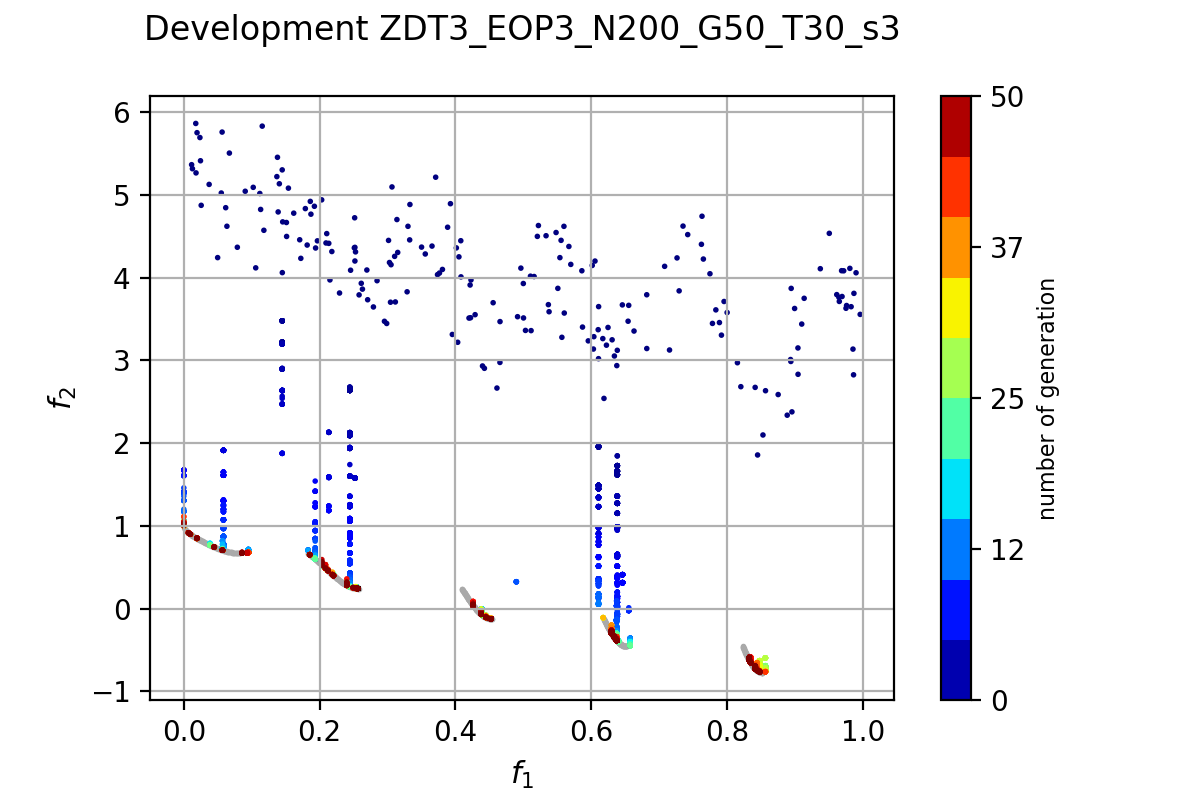
\includegraphics[scale=0.4]{figures/ZDT3_EOP3_N200_G50_T30/s3_dev.png}\\
        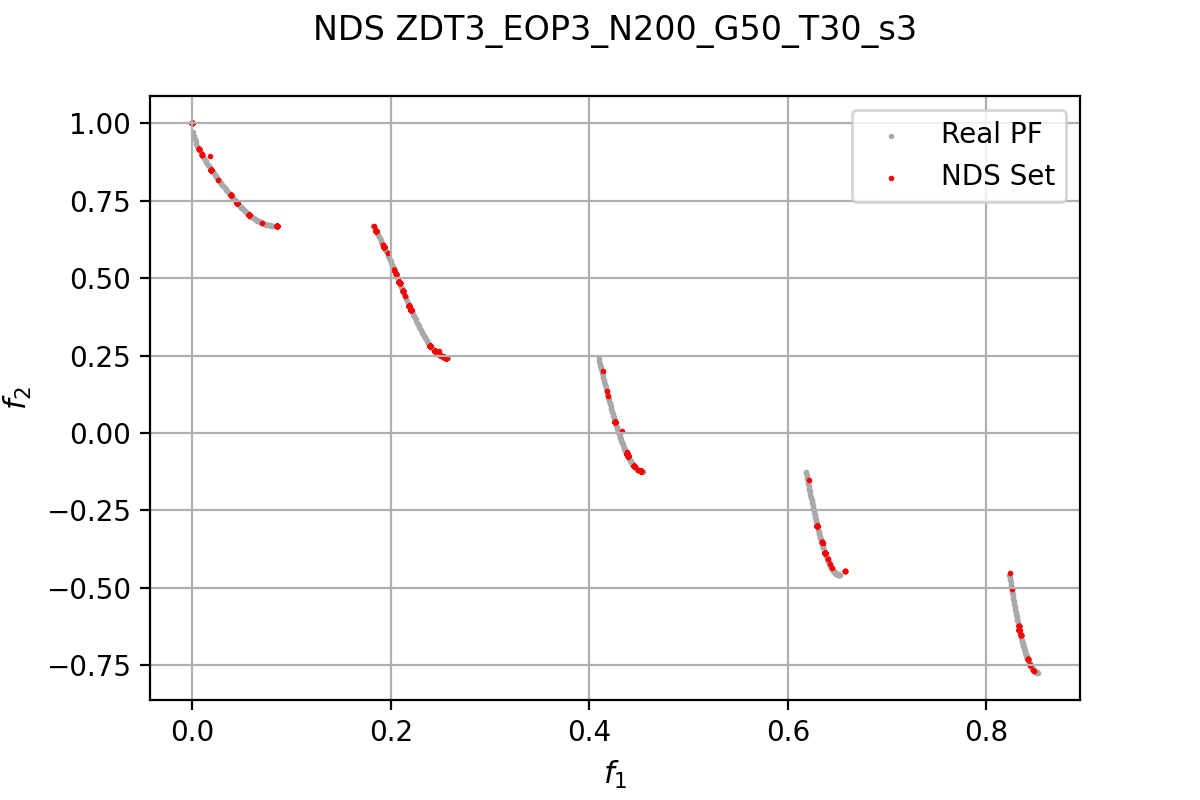
\includegraphics[scale=0.36]{figures/ZDT3_EOP3_N200_G50_T30/s3_nds.png}\\
        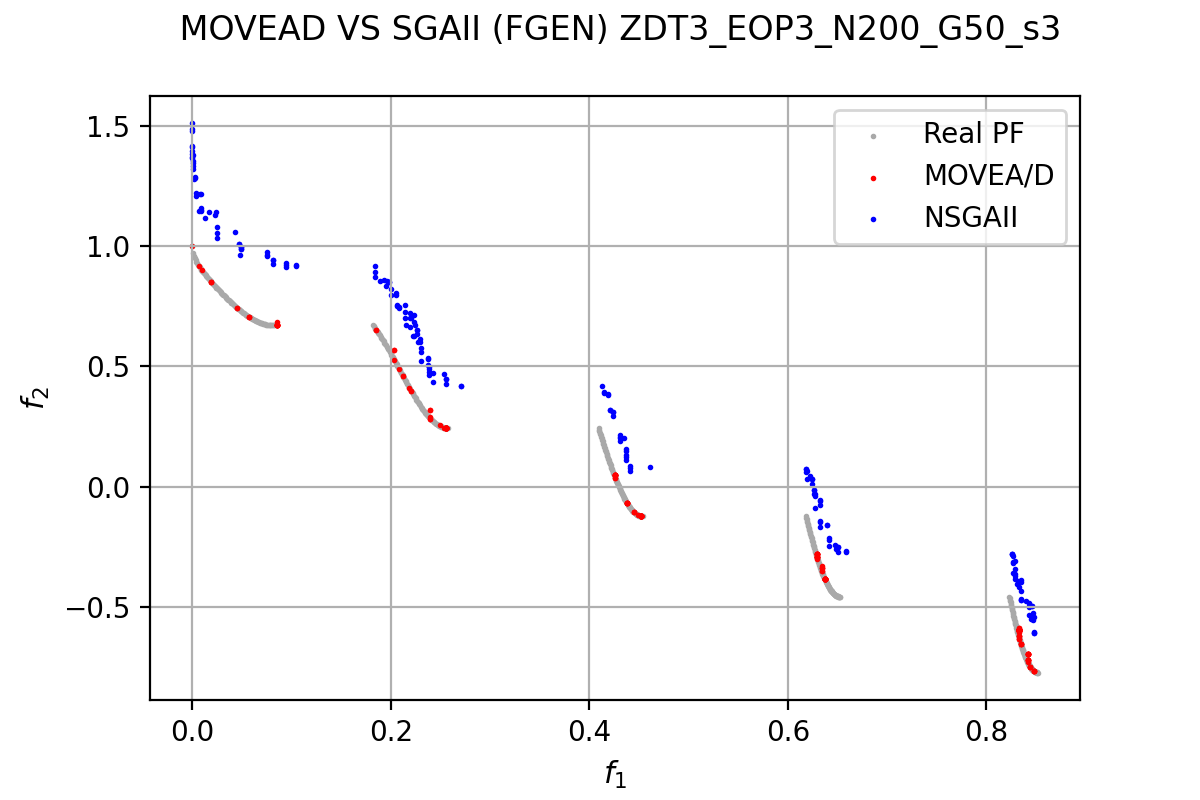
\includegraphics[scale=0.36]{figures/ZDT3_EOP3_N200_G50_T30/s3_comp.png}\\
        \caption{\centering MOEA/D + EOP3 (N200G50)}
        \label{fig:20}
    \end{figure}
    \end{minipage}\\
\end{minipage}\\

Finalmente vamos a realizar una comparativa entre los tres casos tanto para los frentes de la última generación como para los frentes \textit{NSD}. En la \hyperref[fig:21]{\textit{figura 21}} se muestran las dos gráficas de comparativa de los frente anteriormente indicados. En cuanto a las soluciones de la generación final todas se encuentran bastante superpuestas, en cuanto a convergencia todos tienen un comportamiento muy parecido, y quizá la el frente rojo, correspondiente al tercer caso denote una mejor cobertura del frente. En cuanto al NSD las sensaciones son análoga sy nada concluyentes, así que intentaremos clarificarlos con el uso de métricas y el correspondiente estudio estadístico de las mismas.\\ 

\begin{center}
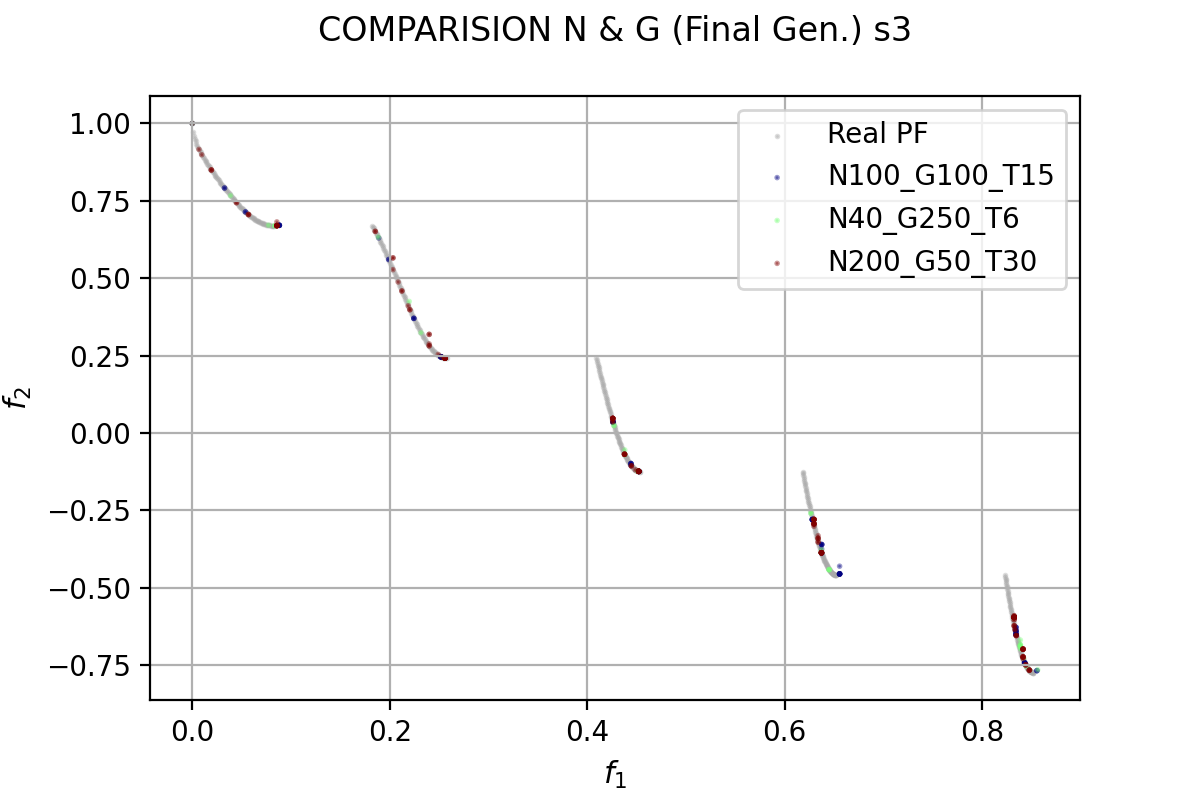
\includegraphics[scale=0.8]{figures/COMPARISIONS_EOP3/GCOMP_FGEN_s3.png}\\
\end{center}
\begin{figure}[H]
\centering
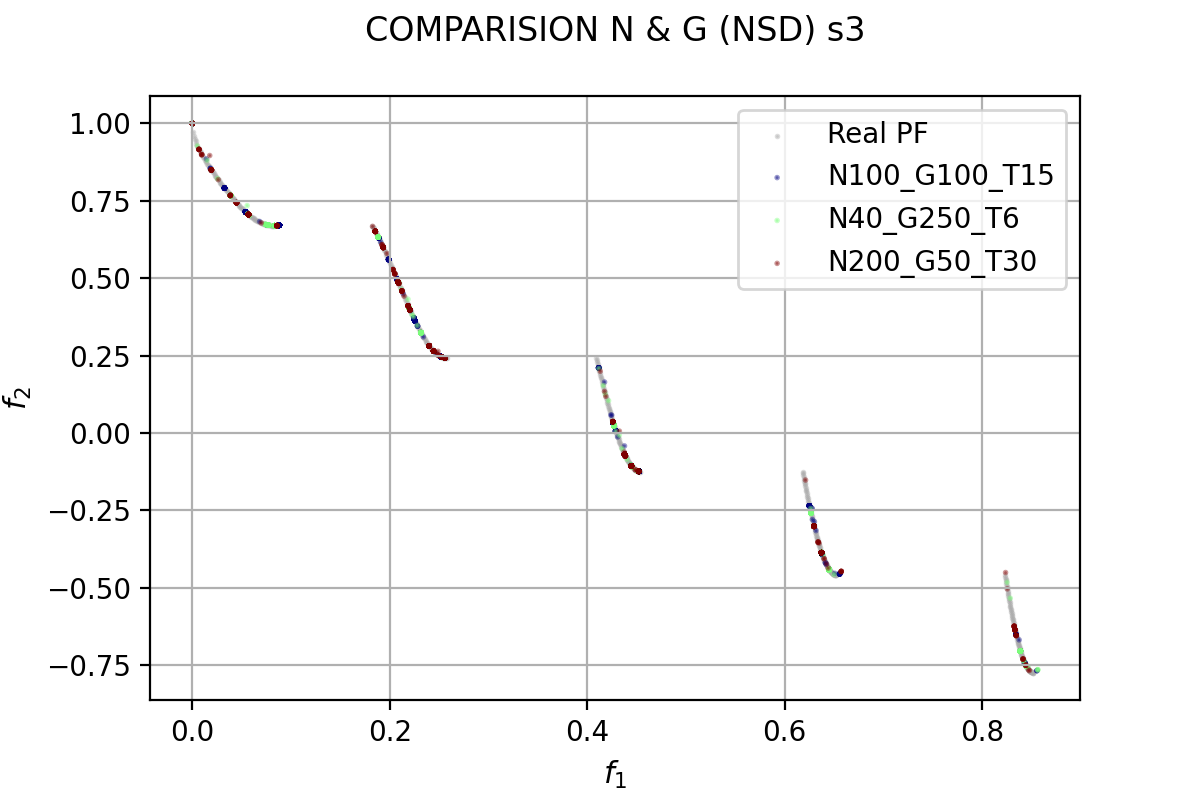
\includegraphics[scale=0.8]{figures/COMPARISIONS_EOP3/GCOMP_NDS_s3.png}\\
\caption{MOEA/D + EOP3. Comparación de casos}
\label{fig:21}
\end{figure}



\subsubsection{Análisis de métricas para 10000 ev.}

Presentado el estudio preliminar anterior vamos a tratar de profundizar para exclarecer y llevar a cabo una discusión más profunda de los casos anteriores. Para ello realizaremos un estudio de algunas métricas para los casos ya presentados. Tales métricas corresponden al hipervolumen, espaciado y cover set.\\

Comencemos viendo algunas gráficas asociadas a las métricas para los casos planteados en el apartado anterior. En la \hyperref[fig:22]{figura 22} se muestra la evolución de hipervolumen y el espaciado en durante las distintas generaciones para 10 ejecuciones del algoritmo. Podemos observar que en todos los casos tanto el desarrollo del hipervolumen como el de el espaciado se comporta de forma bastante uniforme para todas las ejecuciones.\\

Aunque no es posible hacer un análisis conjunto del hipervolumen (ya que el punto de referencia para su cálculo es distinto en cada caso) sí podemos destacar la rápida convergencia del algoritmo, beneficiándose también del número de subproblemas más que de el número de generaciones observando una tendencia de estancamiento a partir de en torno al 40\% de las generaciones, en los tres casos. Observando además el beneficio del incremento del número de subproblemas en el espaciado, cuyo valor suele tender a disminuir con dicho aumento, de forma que parece claro que es preferible dedicar (de forma razonable) más parte de la potencia computacional al número de subproblemas en vez de al número de generaciones. \\

\begin{center}
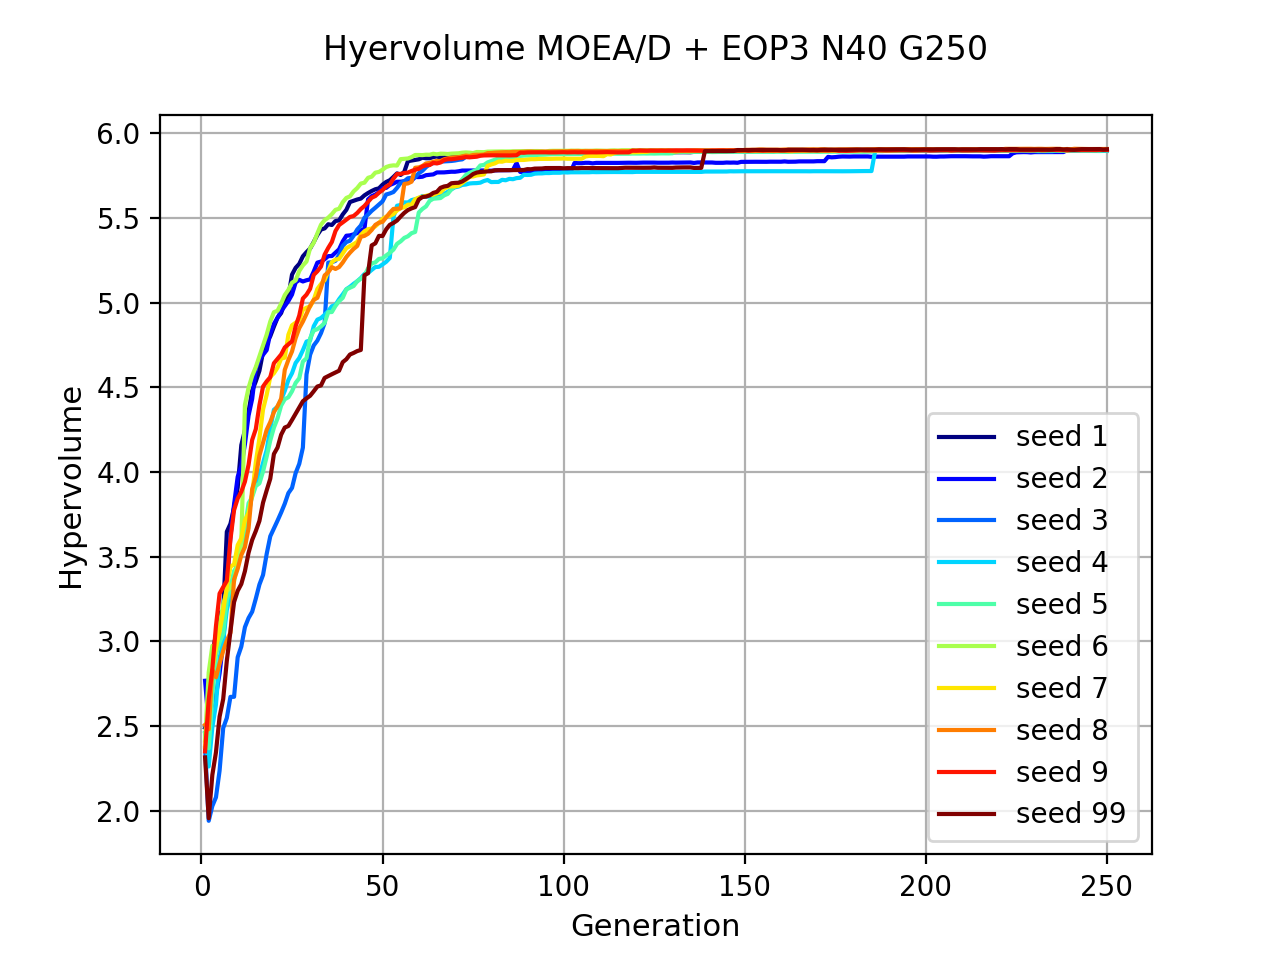
\includegraphics[scale=0.5]{figures/METRICS_EOP3/Hypervol_N40_G250.png}\quad 
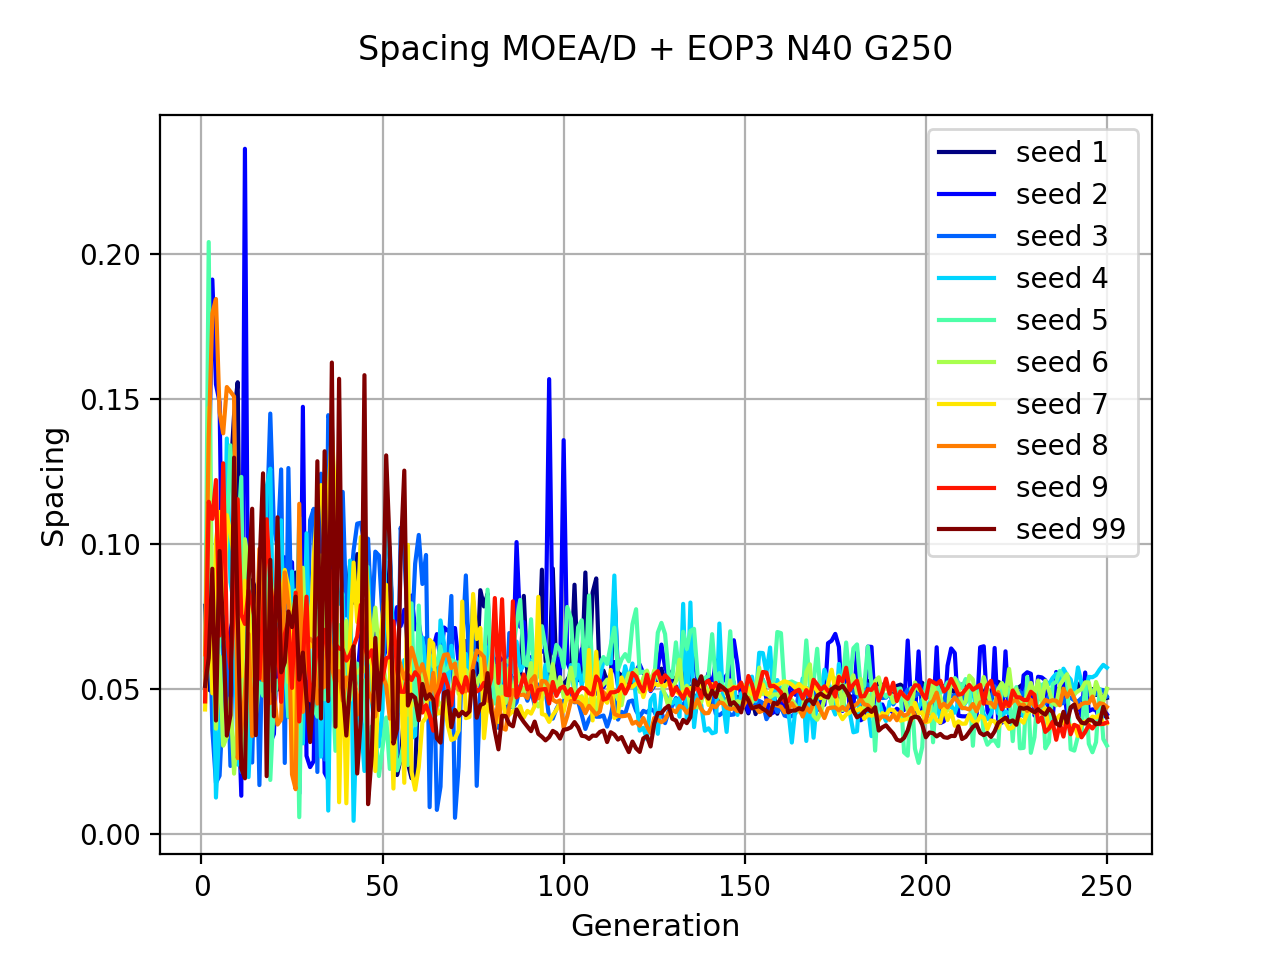
\includegraphics[scale=0.5]{figures/METRICS_EOP3/Spacing_N40_G250.png}\\
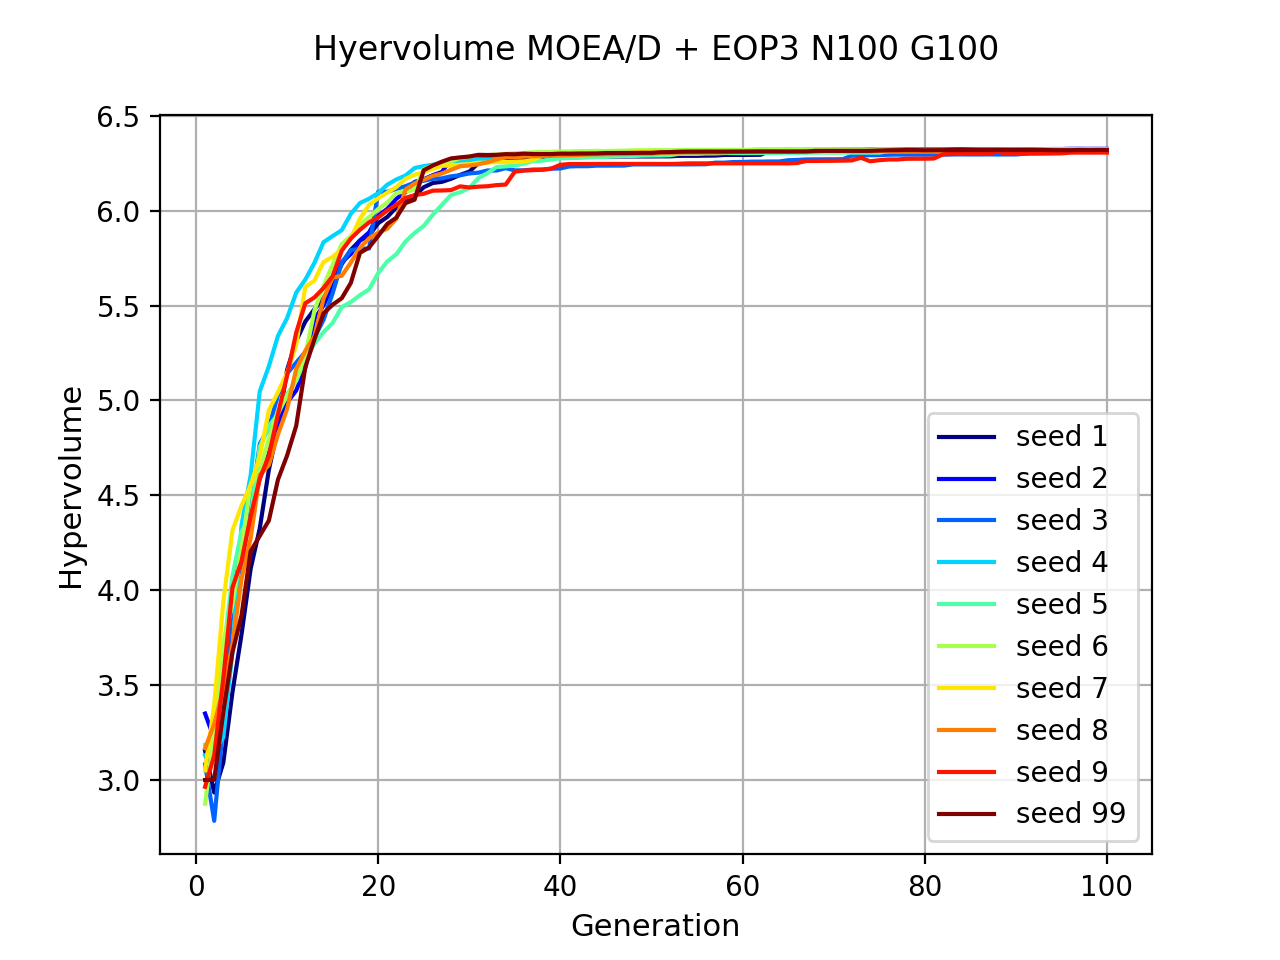
\includegraphics[scale=0.5]{figures/METRICS_EOP3/Hypervol_N100_G100.png} \quad 
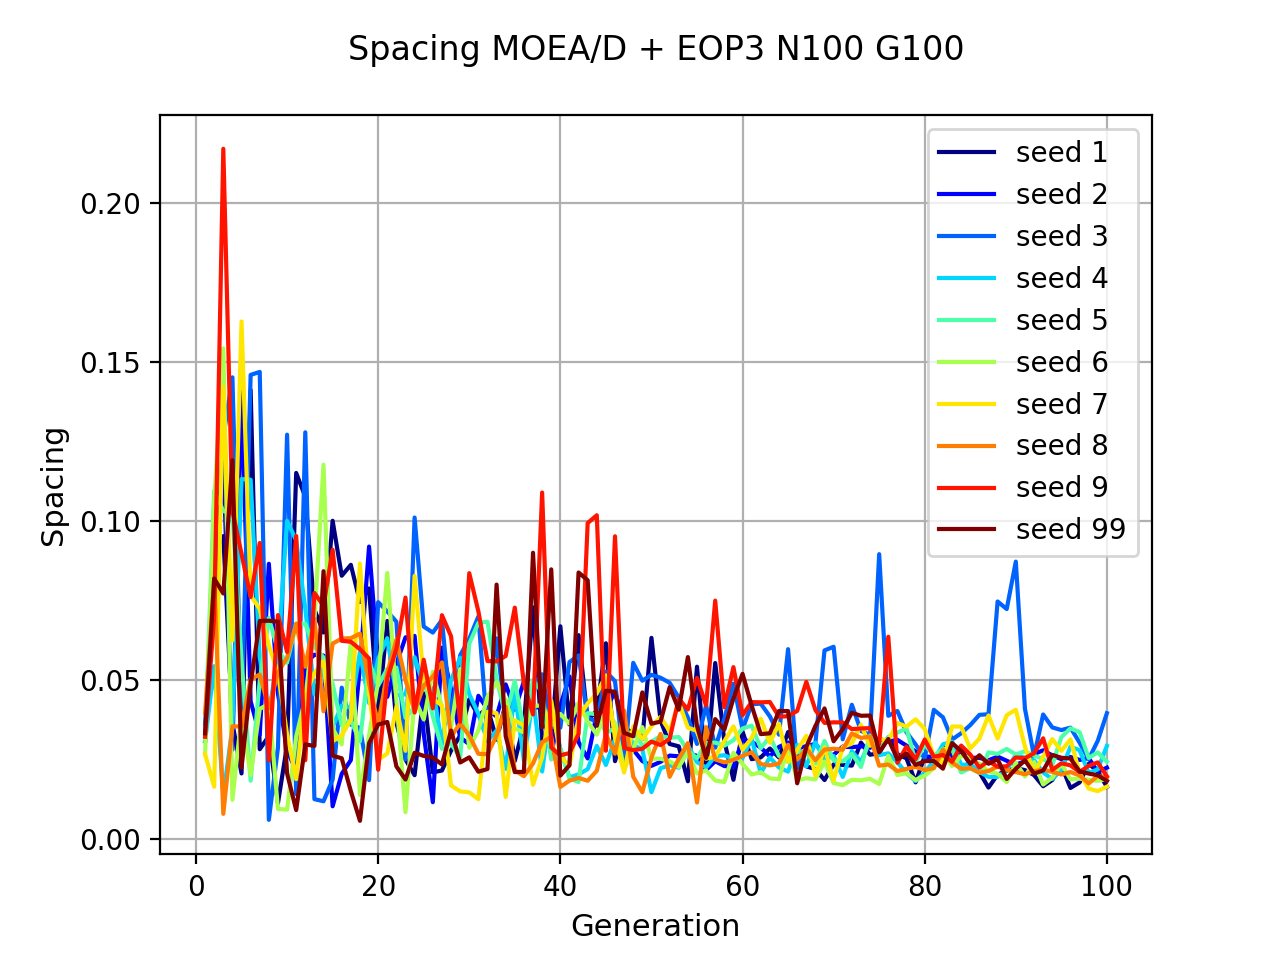
\includegraphics[scale=0.5]{figures/METRICS_EOP3/Spacing_N100_G100.png}\\
\end{center}

\begin{figure}[H]
\centering
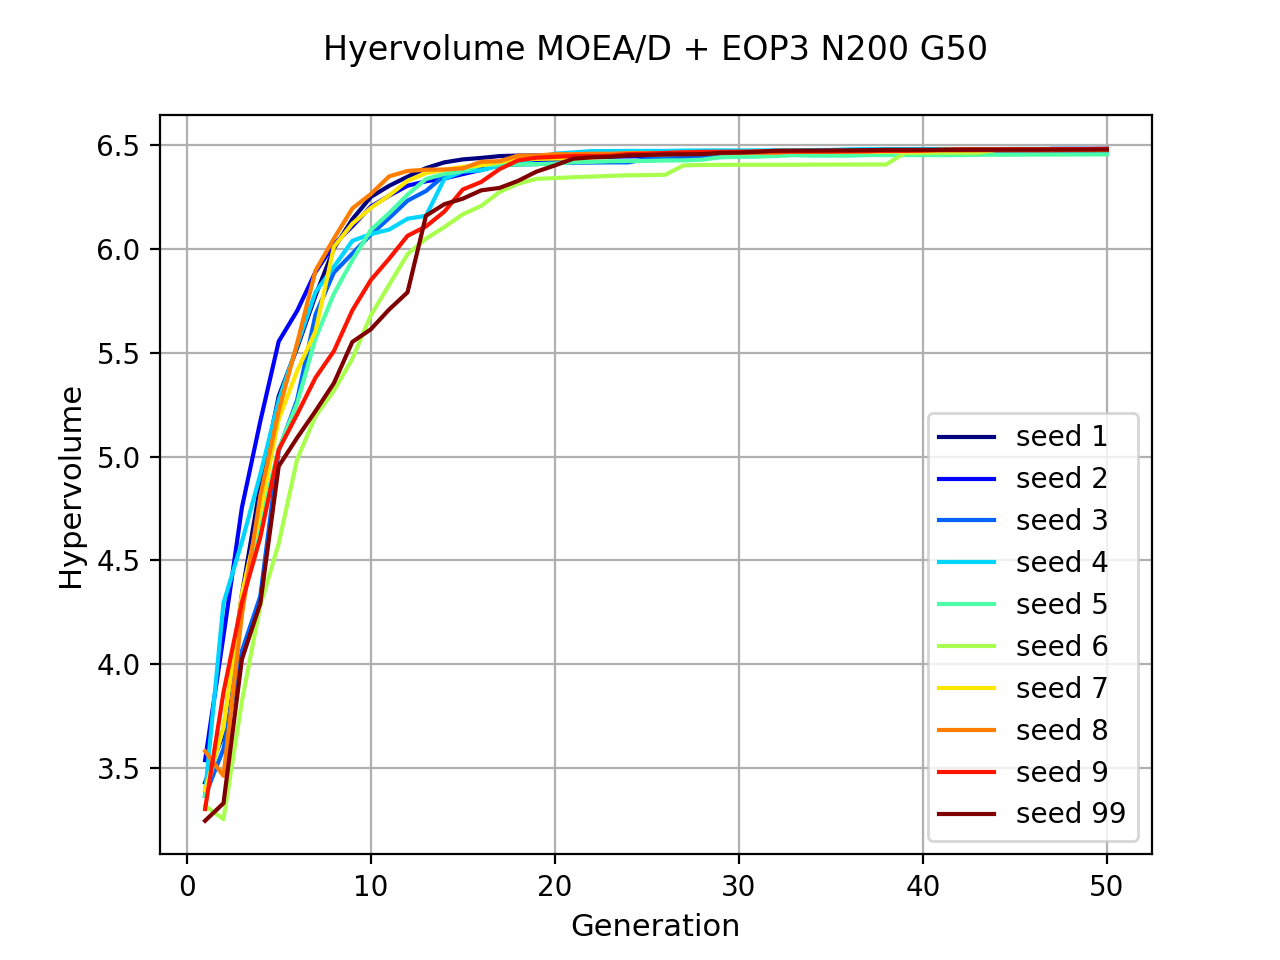
\includegraphics[scale=0.5]{figures/METRICS_EOP3/Hypervol_N200_G50.png}\quad 
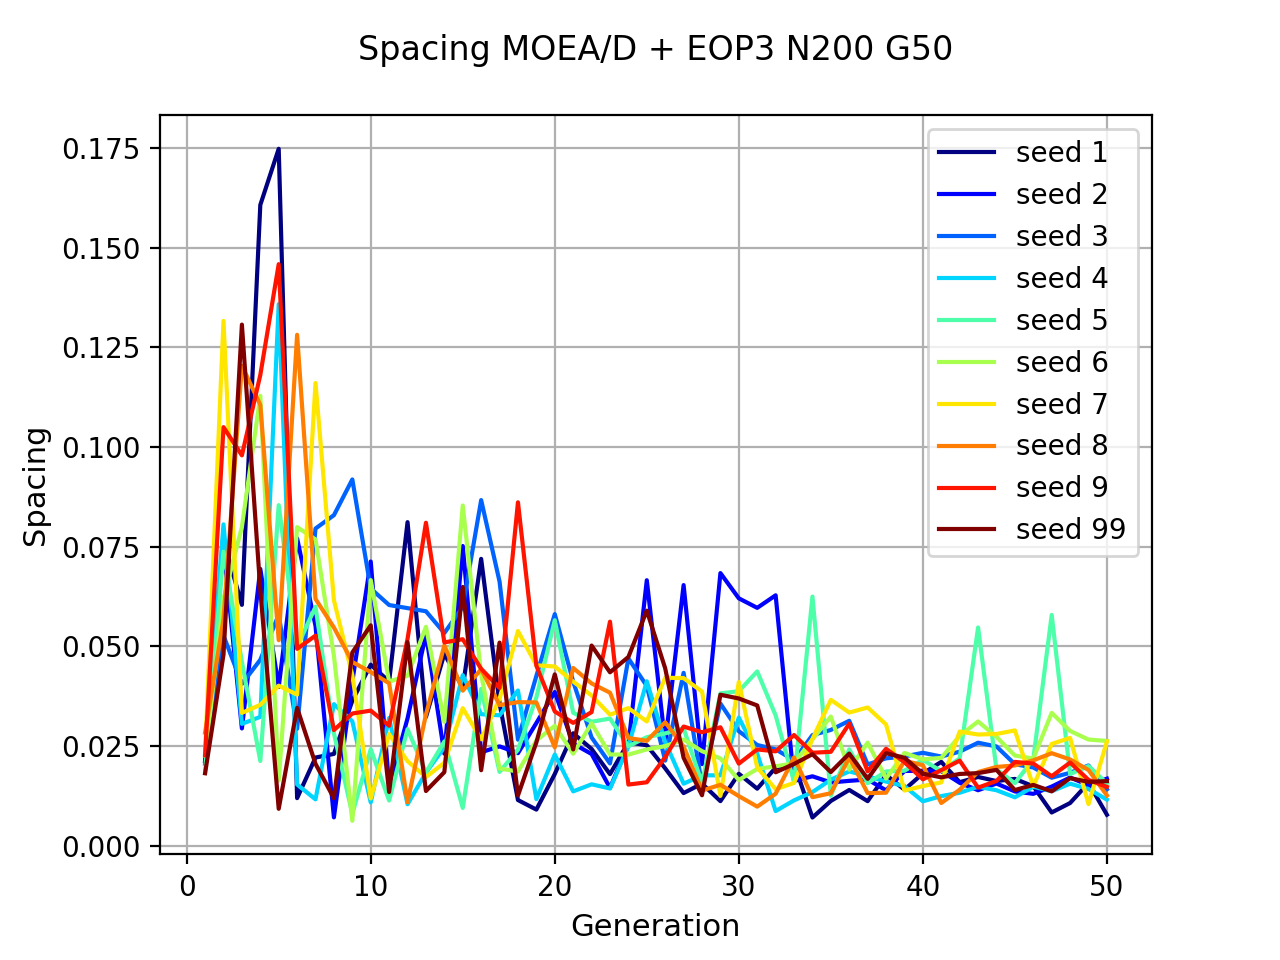
\includegraphics[scale=0.5]{figures/METRICS_EOP3/Spacing_N200_G50.png}\\
\caption{MOEA/D + EOP3. Méticas para 10000 EV}
\label{fig:22}
\end{figure}


\begin{figure}[H]
\centering
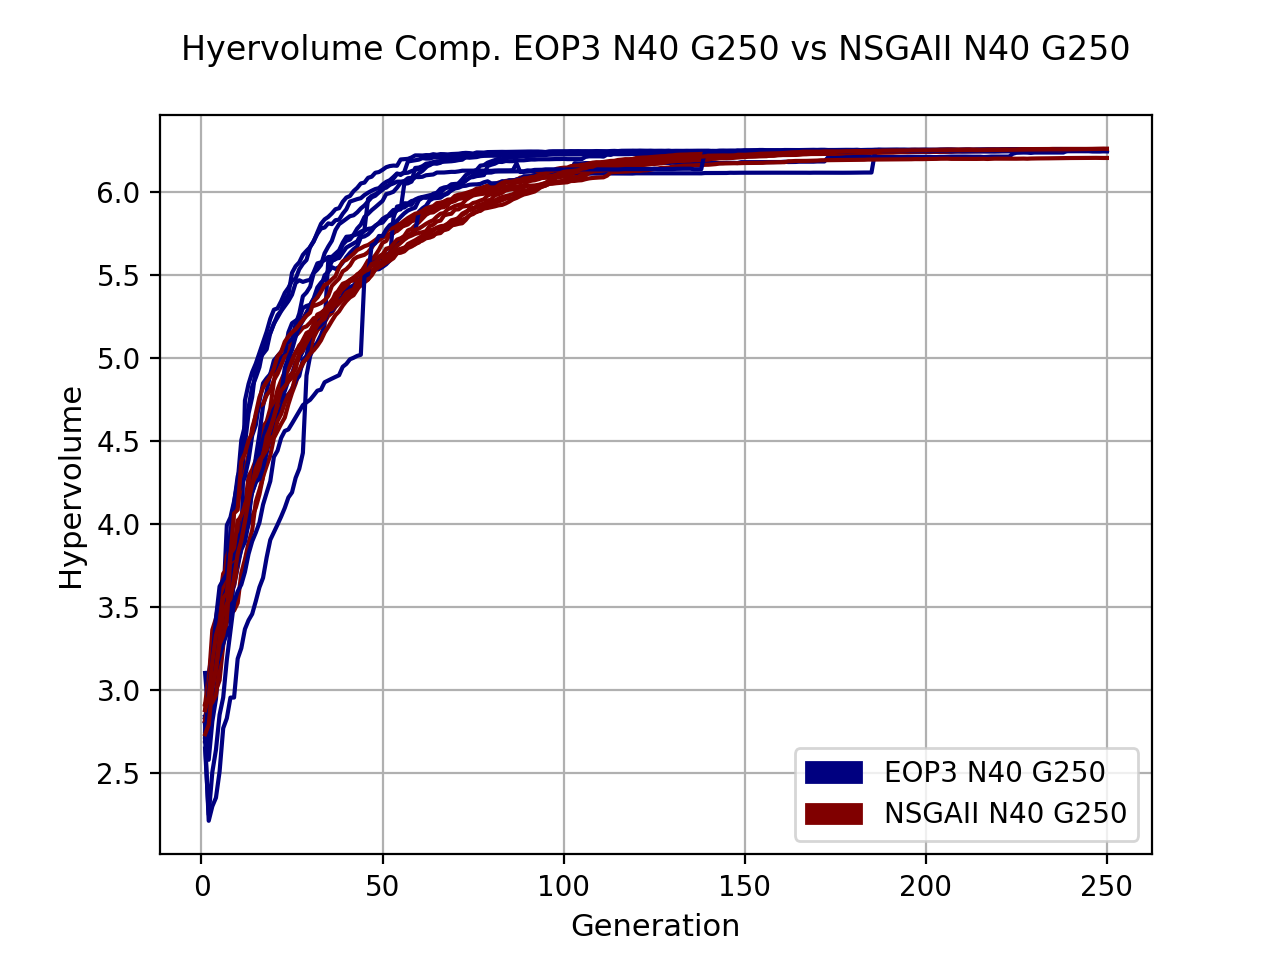
\includegraphics[scale=0.35]{../METRICS_PLOTS/Hypervol_COMP_EOP3N40G250_NSGAIIN40G250.png}
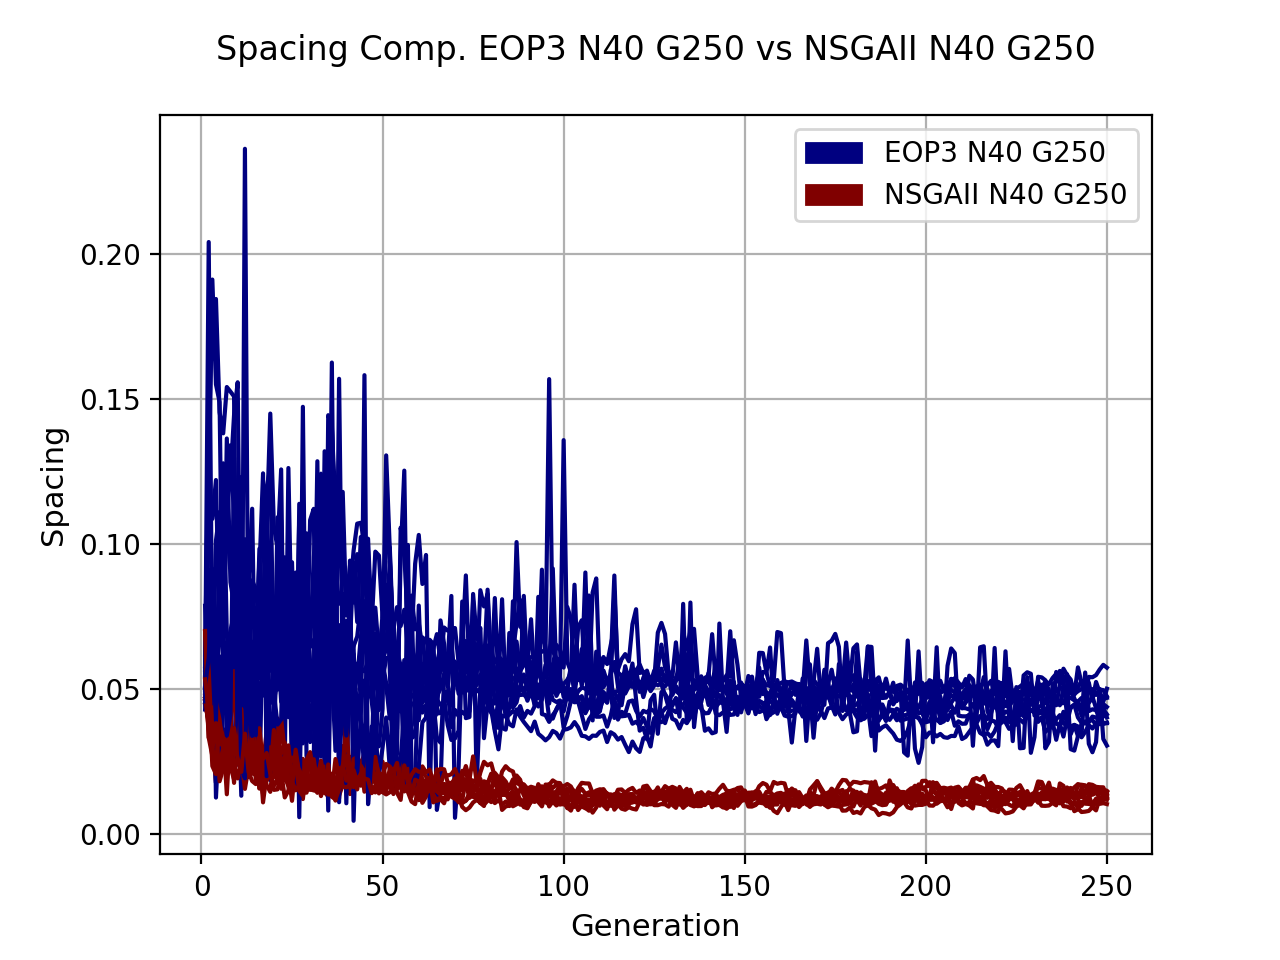
\includegraphics[scale=0.35]{../METRICS_PLOTS/Spacing_COMP_EOP3N40G250_NSGAIIN40G250.png}
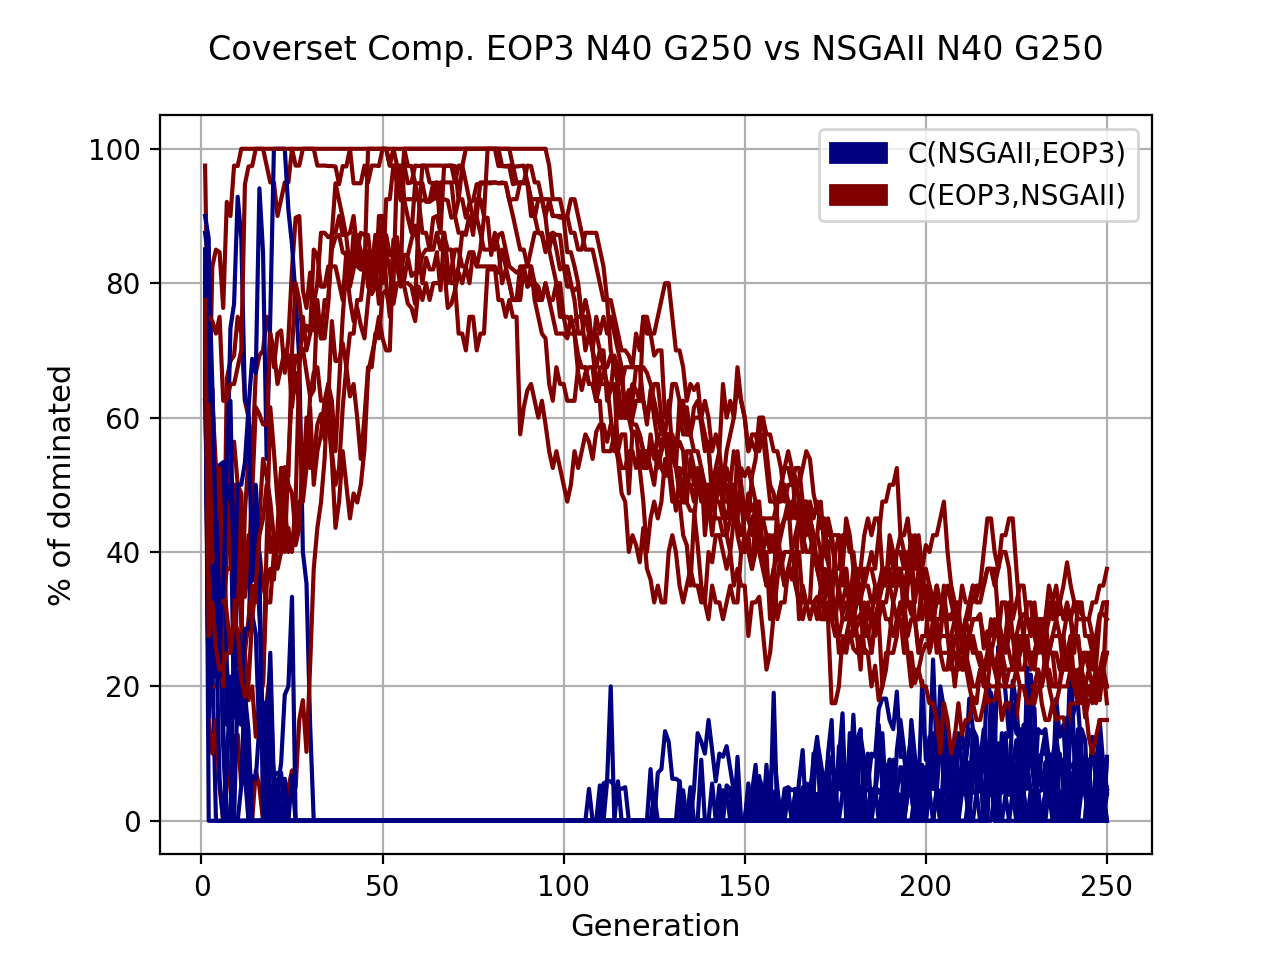
\includegraphics[scale=0.35]{../METRICS_PLOTS/CoverSet_COMP_EOP3N40G250_NSGAIIN40G250.png}\\
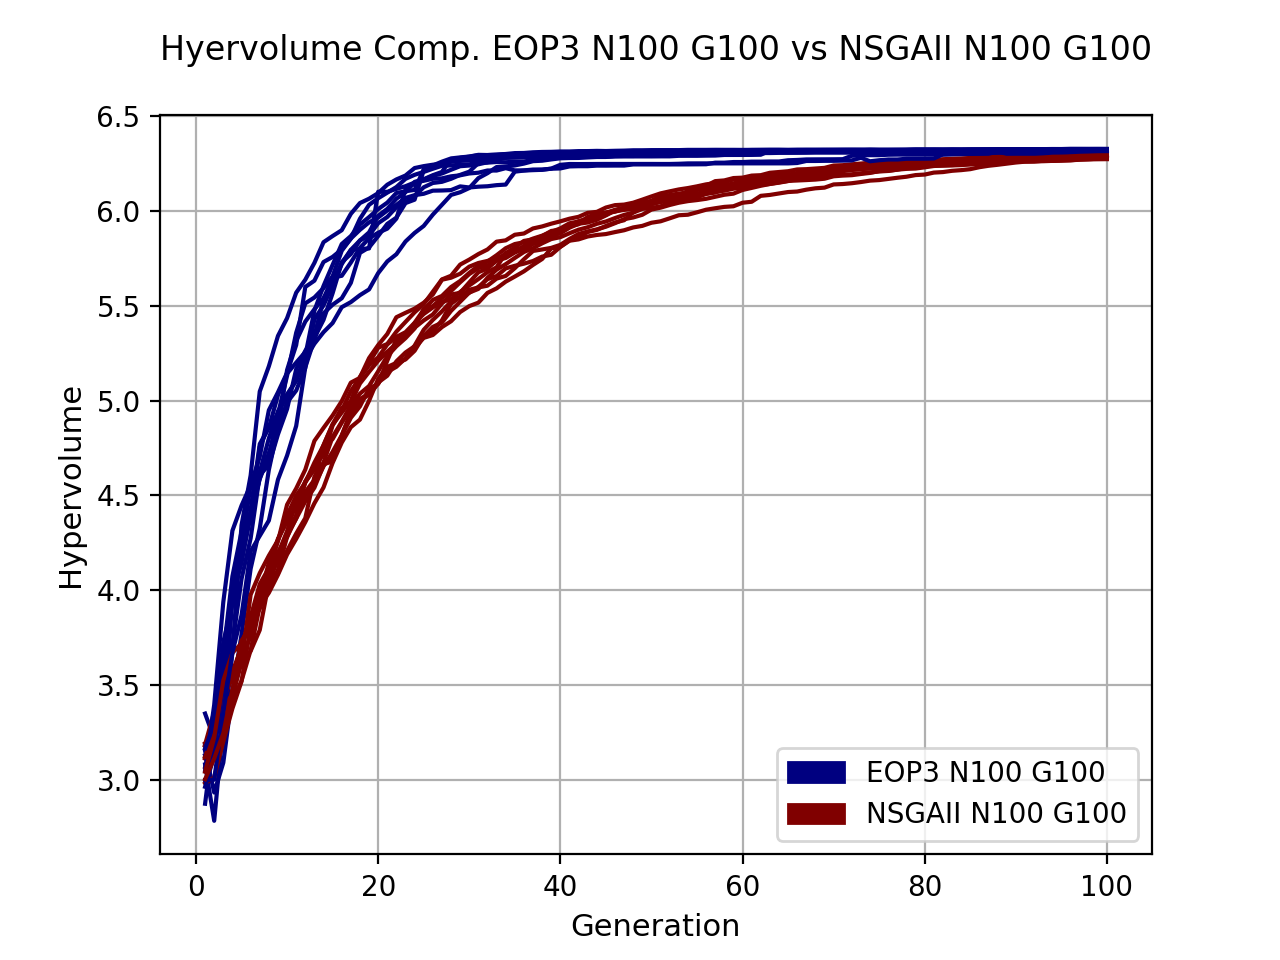
\includegraphics[scale=0.35]{../METRICS_PLOTS/Hypervol_COMP_EOP3N100G100_NSGAIIN100G100.png}
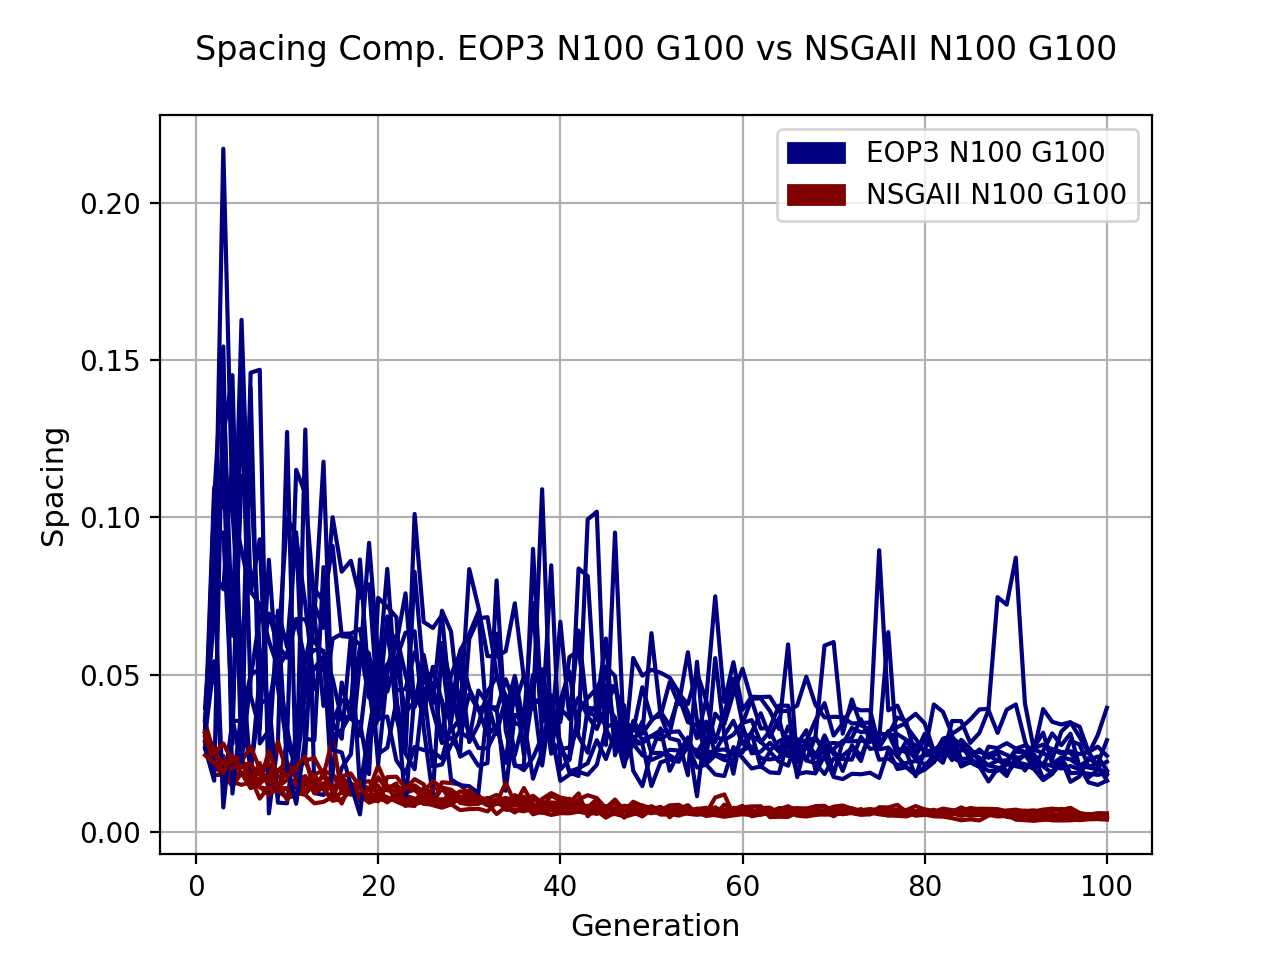
\includegraphics[scale=0.35]{../METRICS_PLOTS/Spacing_COMP_EOP3N100G100_NSGAIIN100G100.png}
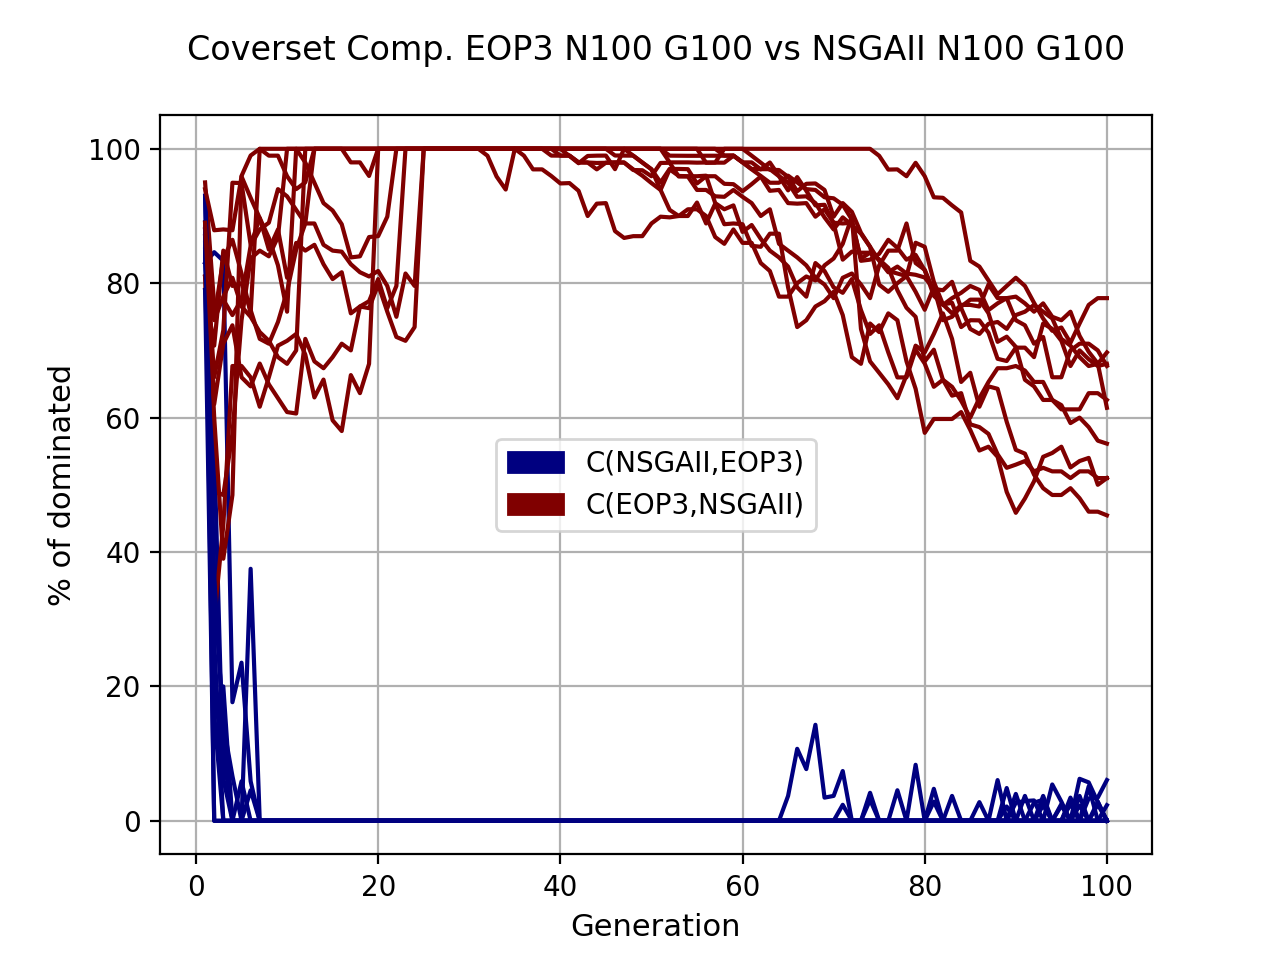
\includegraphics[scale=0.35]{../METRICS_PLOTS/CoverSet_COMP_EOP3N100G100_NSGAIIN100G100.png}\\
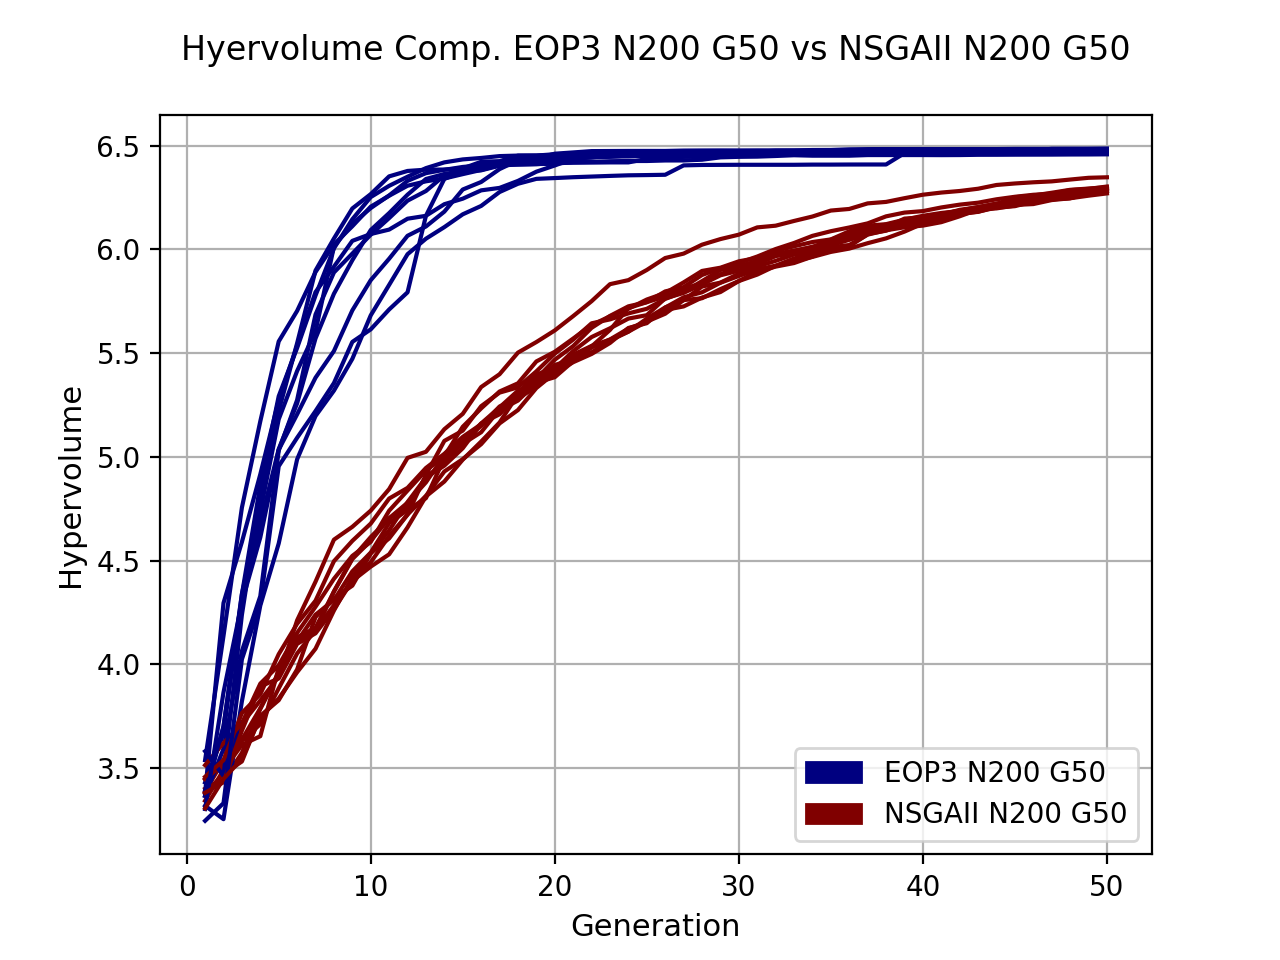
\includegraphics[scale=0.35]{../METRICS_PLOTS/Hypervol_COMP_EOP3N200G50_NSGAIIN200G50.png}
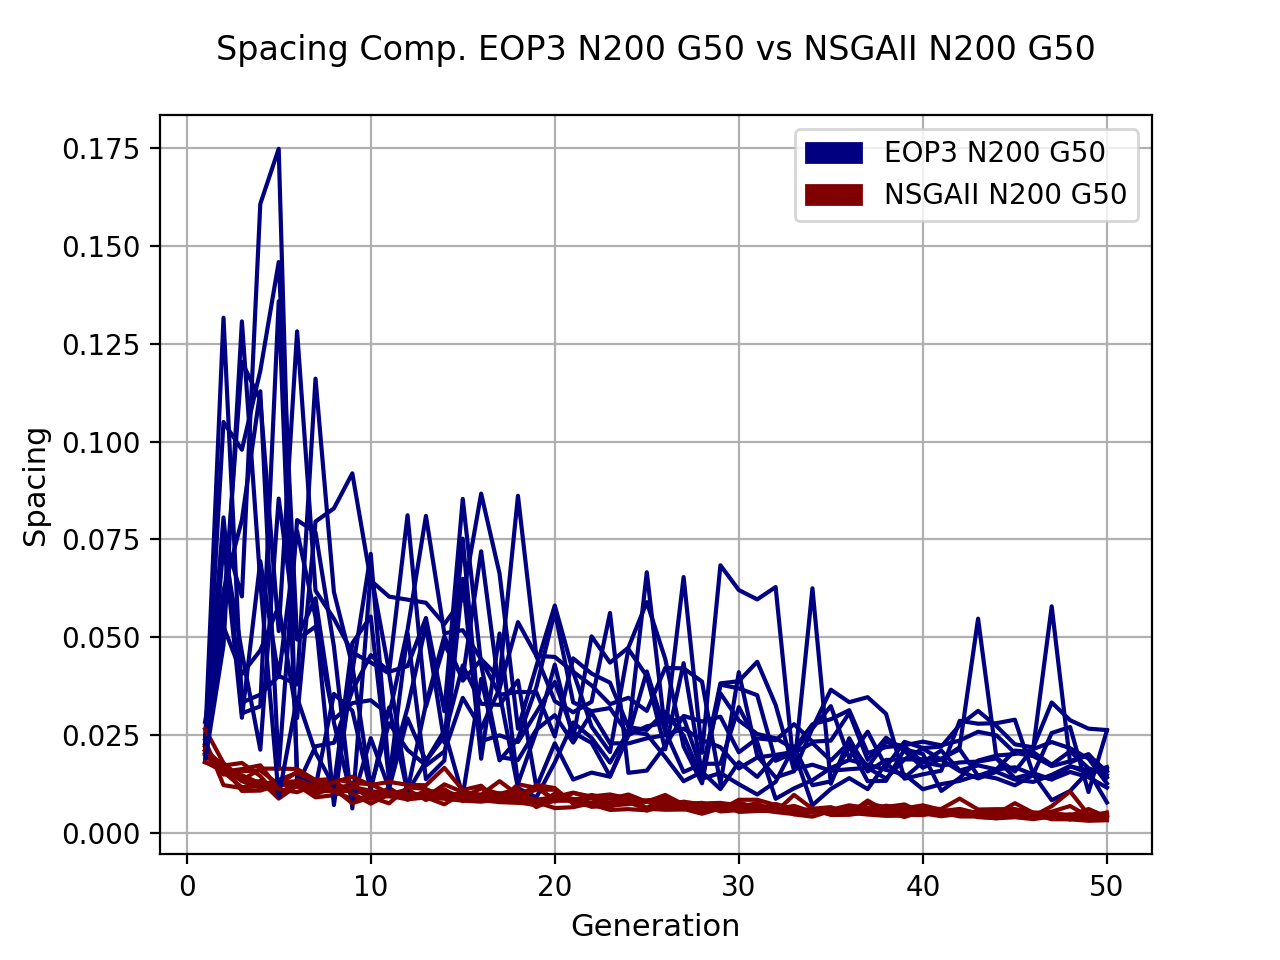
\includegraphics[scale=0.35]{../METRICS_PLOTS/Spacing_COMP_EOP3N200G50_NSGAIIN200G50.png}
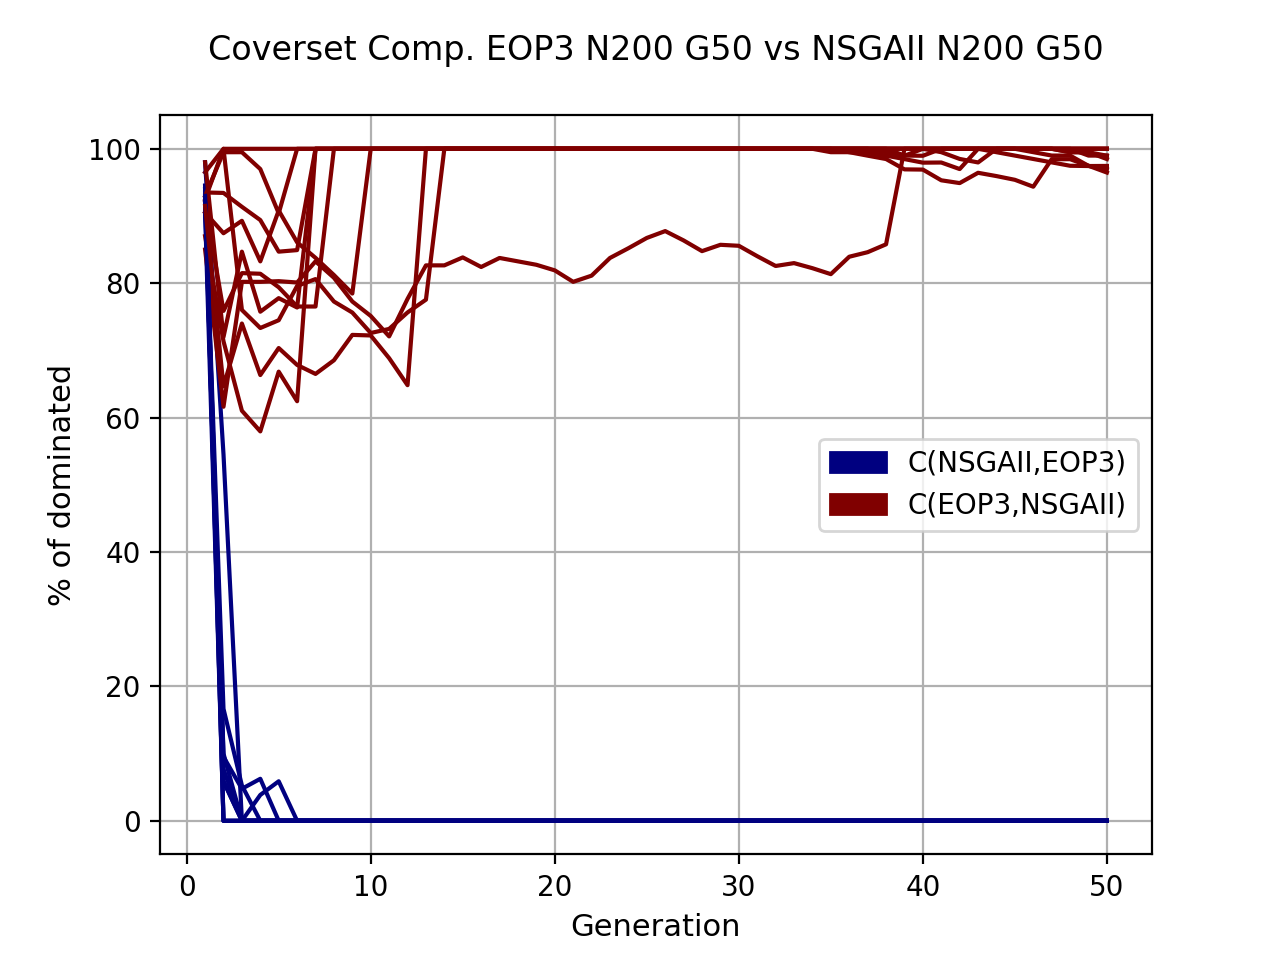
\includegraphics[scale=0.35]{../METRICS_PLOTS/CoverSet_COMP_EOP3N200G50_NSGAIIN200G50.png}\\
\caption{MOEA/D + EOP3. Comparación de métricas con NSGAII para 10000 EV.}
\label{fig:23}
\end{figure}

A continuación presentaremos algunas gráficas comparativas del comportamiento del algoritmo frente a \textit{NSGAII}. En la \hyperref[fig:23]{figura 23} se muestran las graficas con dichas comparativas en las que podemos notar que en todos los casos el espaciado en el algoritmo \textit{NSGAII} se comporta mejor que en algoritmo propuesto mientras que el hipervolumen el comportamiento es el contrario de forma muy notable para los casos con más subproblemas. Como vimos en el estudio preliminar el algoritmo, con los suficientes subproblemas, sí suele converger a soluciones mejores que el algoritmo \textit{NSGAII} pero también suele tender a concentrar más las soluciones.\\

Sin embargo si comprobamos la métrica cover set, sí podemos ver que en el primer caso ninguno de los frentes es dominado más de un 40\% por el otro en la mayoría de las ejecuciones, pero aún así nuestro algoritmo queda en todos los casos por debajo, no superando para ninguna de las ejecuciones el 17\% de dominancia. Para el segundo y tercer caso la situación es mucho clara, de forma que en casi todas las ejecuciones el frente del algoritmo \textit{NSGAII} quedó dominado por el de \textit{MOEA/D + EOP2} entre el 50\% y el 80\% de sus puntos, mientras que el frente de  \textit{NSGAII} domina al \textit{MOEA/D + EOP2} en menos de un 10\% en todas de las ejecuciones y para el tercer caso, el frente de \textit{NSGAII} queda dominado por el de nuestro algoritmo en más de un 95\% en todas las ejecuciones mientras que el caso contrario no es apreciable para ningún punto de ninguna de las ejecuciones (en más de 1\% o 2\%). De forma que queda patente los resultados que ya comentamos para el operador EOP1 pero que en este caso se manifiestan con mayor relevancia, la cantidad de subproblemas es mucho más beneficiosa que la cantidad de generaciones.\\

Aunque en este apartado no hemos realizado (explícitamente) un análisis de las soluciones (población final y NSD) en el último apartado de esta sección presentaremos una comparativa conjunta de las últimas generaciones y de los conjuntos no dominados (NSD) para todos los casos y todos los algoritmos.	\\

\noindent\textbf{EXPERIMENTACIÓN PARA 4000 EVALUACIONES}\\

Ya presentamos para 10000 evaluaciones el comportamiento del algoritmo es adecuado, esto es, a través de las generaciones los individuos se aproximan al frente. No vamos a volver a presentarlo para el caso de 4000 evaluaciones, pues sigue lógicamente el mismo esquema (en los apéndices se presentan las gráficas que atestiguan lo expuesto). Por tanto pasaremos directamente a evaluar las métricas y a razonar directamente sobre los resultados obtenidos en dicho análisis.  \\

En la \hyperref[fig:24]{figura 24} se presentan las gráficas del desarrollo del hypervolumen y el espaciado para cada uno de los casos coniderados en las 4000 evaluaciones en contreto $(N=40, G=100)$, $(N=80, G=50)$, $(N=100, G=40)$. Como podemos apreciar el comportamiento es similar a los presentados para las 10000 evaluaciones, de hecho se empieza a atisvar la mencionada llegada a la zona de estanco y sí es notable la gran variabilidad del espaciado dada la falta de subproblemas y generaciones, disminuyendo dicha variabilidad ligeramente con el aumento de los subproblemas..\\

Si realizamos una comparativa (al igual que en el caso de 10000 ev) con el algoritmo \textit{NSGAII} obtenemos conclusiones análogas a las presentadas para 10000 evaluaciones, de forma que en el espaciado \textit{NSGAII} supera (valor más bajo) a nuestro algoritmo, aunque sí se denota una mejora con el aumento de los subproblemas. En el caso del hipervolumen nuestro algoritmo supera a \textit{NSGAII} en prácticamente la totalidad de las ejecuciones. En cuanto al cover set,  para el caso $N=40$ más del 50\%  del frente (final) de \textit{NSGAII} es dominado por nuestro algoritmo en todas las ejecuciones, mientras que apenas un no se aprecia (ni un 1\% o 2\%) del caso contrario. En los otros casos la situación es más clara dominando nuestro algoritmo más del 90\% del frente de \textit{NSGAII} en todas las ejecuciones y siendo inapreciable el caso opuesto\\

De todo ello destacamos la bondad de nuestro algoritmo en cuanto a la convergencia, no  para el espaciado  y en cuanto al cover set, con el número adecuado de subproblemas (mejor que de generaciones) nuestro algoritmo domina practicamente en su totalidad a \textit{NSGAII}. Si destacamos frente a EOP1 y EOP2 la severa pérdida de diversidad que lo lleva a un reparto poco uniforme de las soluciones a lo largo del frente.\\

\begin{figure}[H]
\centering
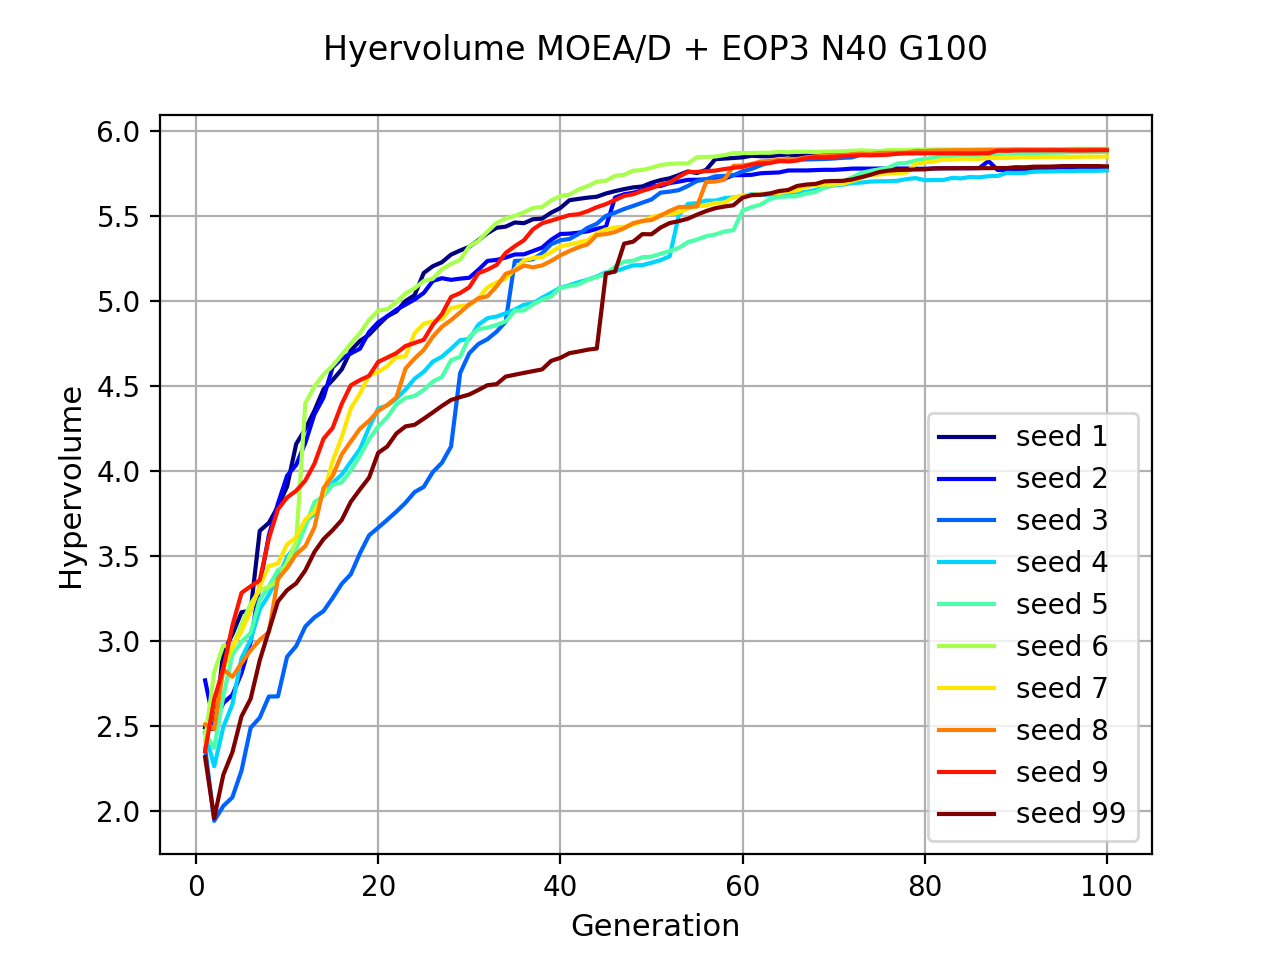
\includegraphics[scale=0.43]{figures/METRICS_EOP3/Hypervol_N40_G100.png} \quad 
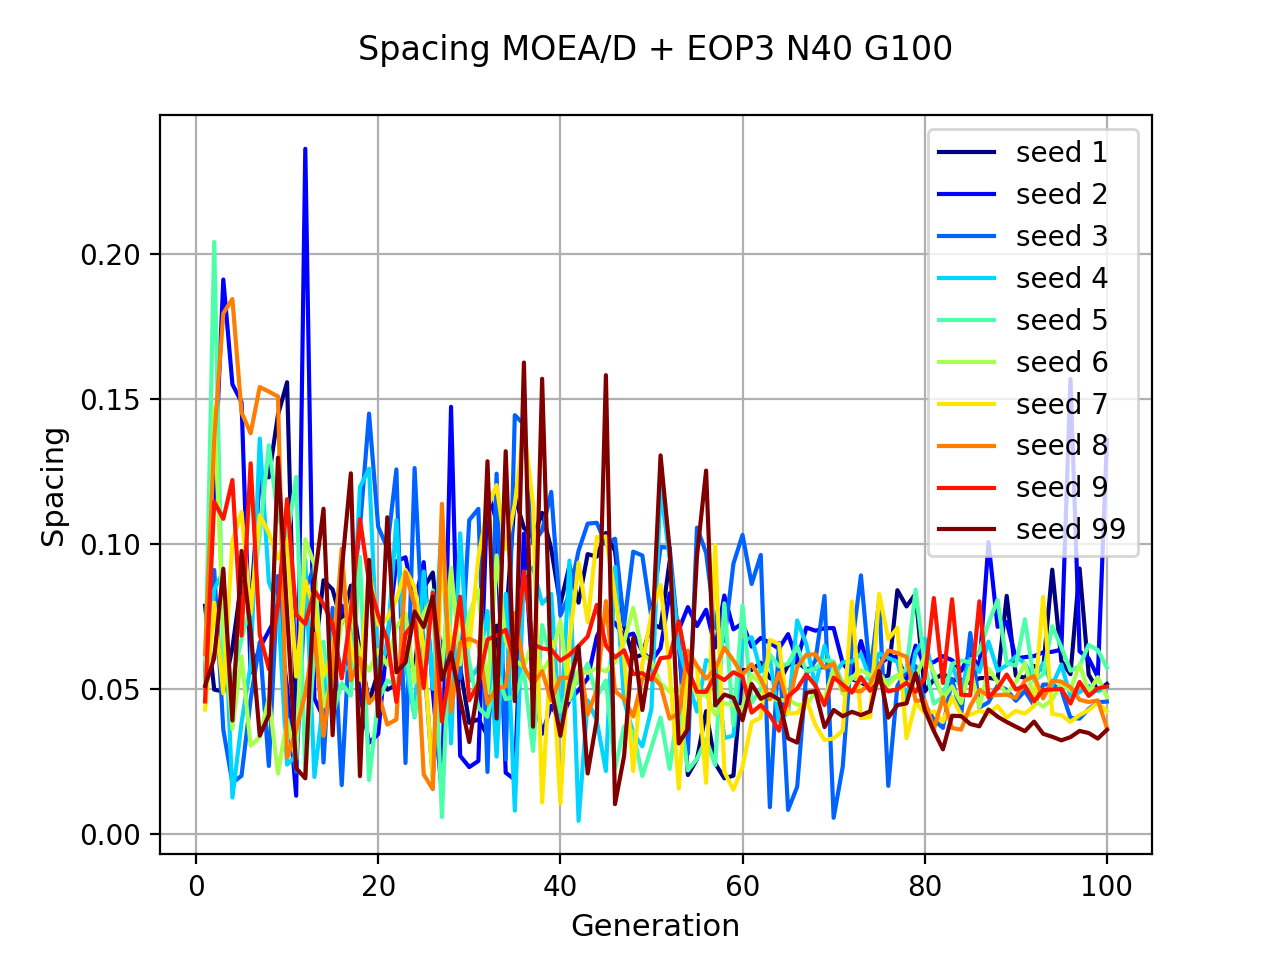
\includegraphics[scale=0.43]{figures/METRICS_EOP3/Spacing_N40_G100.png}\\
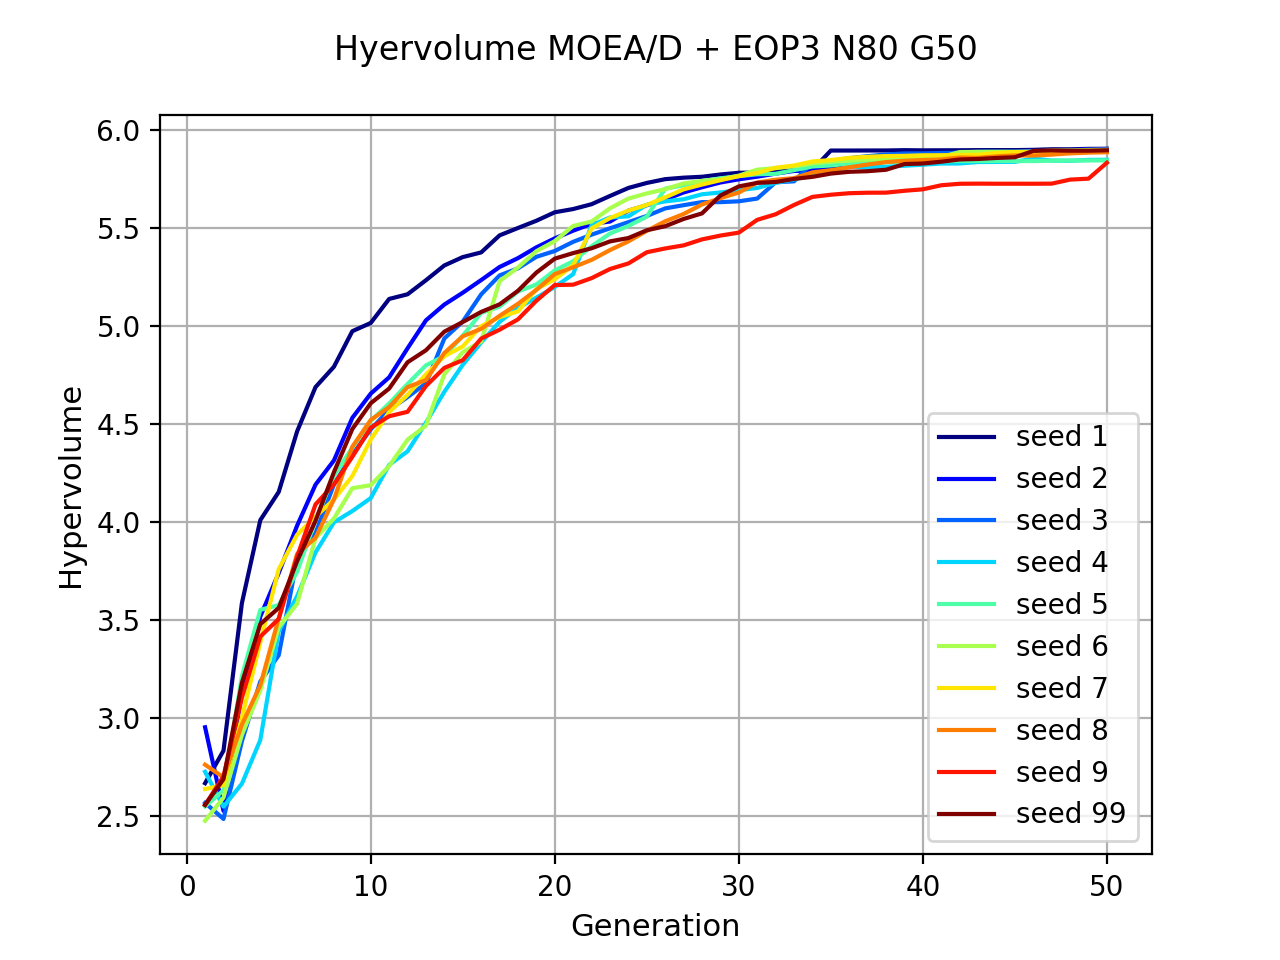
\includegraphics[scale=0.43]{figures/METRICS_EOP3/Hypervol_N80_G50.png}\quad 
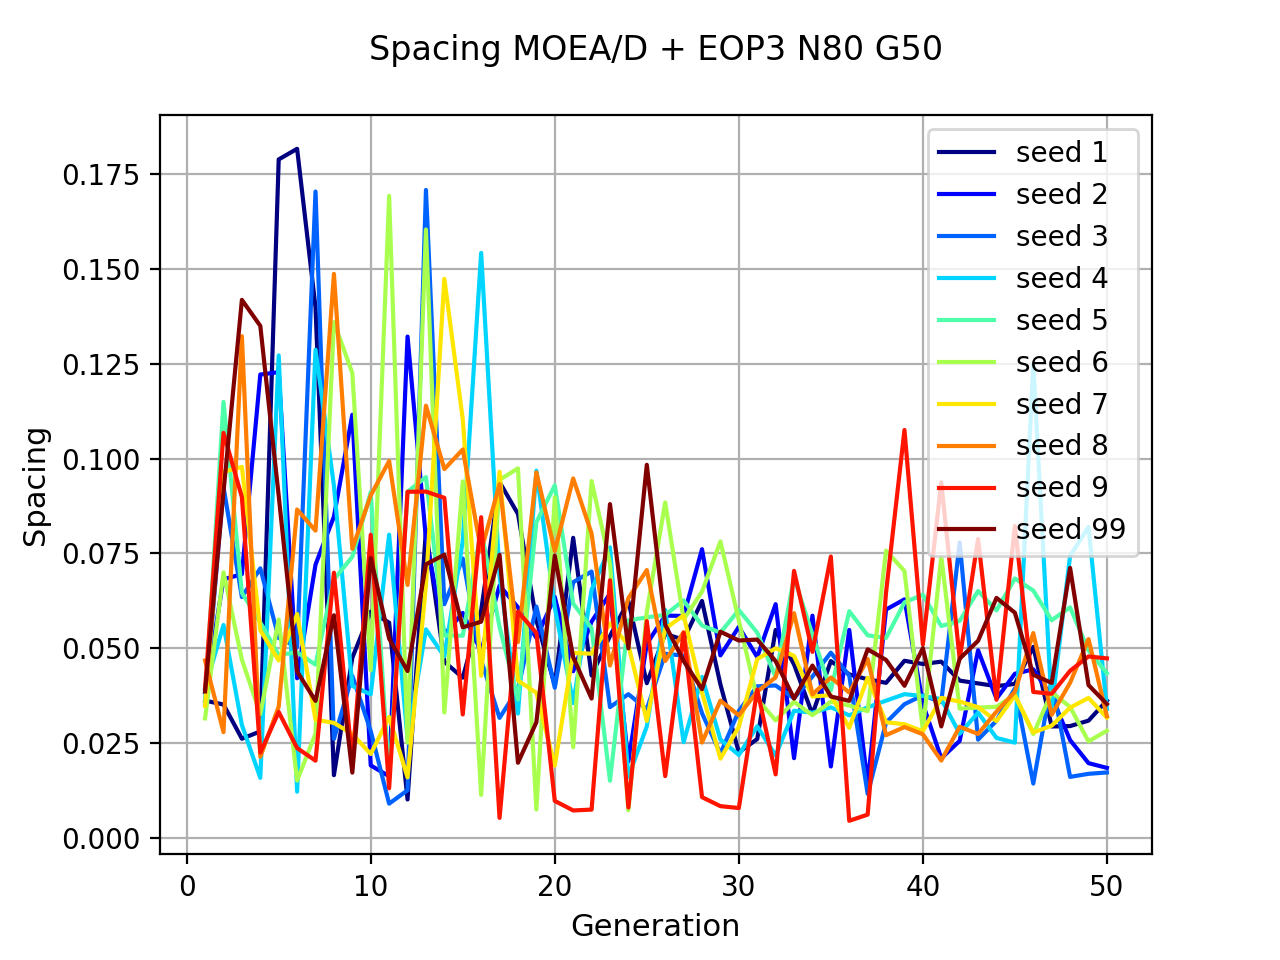
\includegraphics[scale=0.43]{figures/METRICS_EOP3/Spacing_N80_G50.png}\\
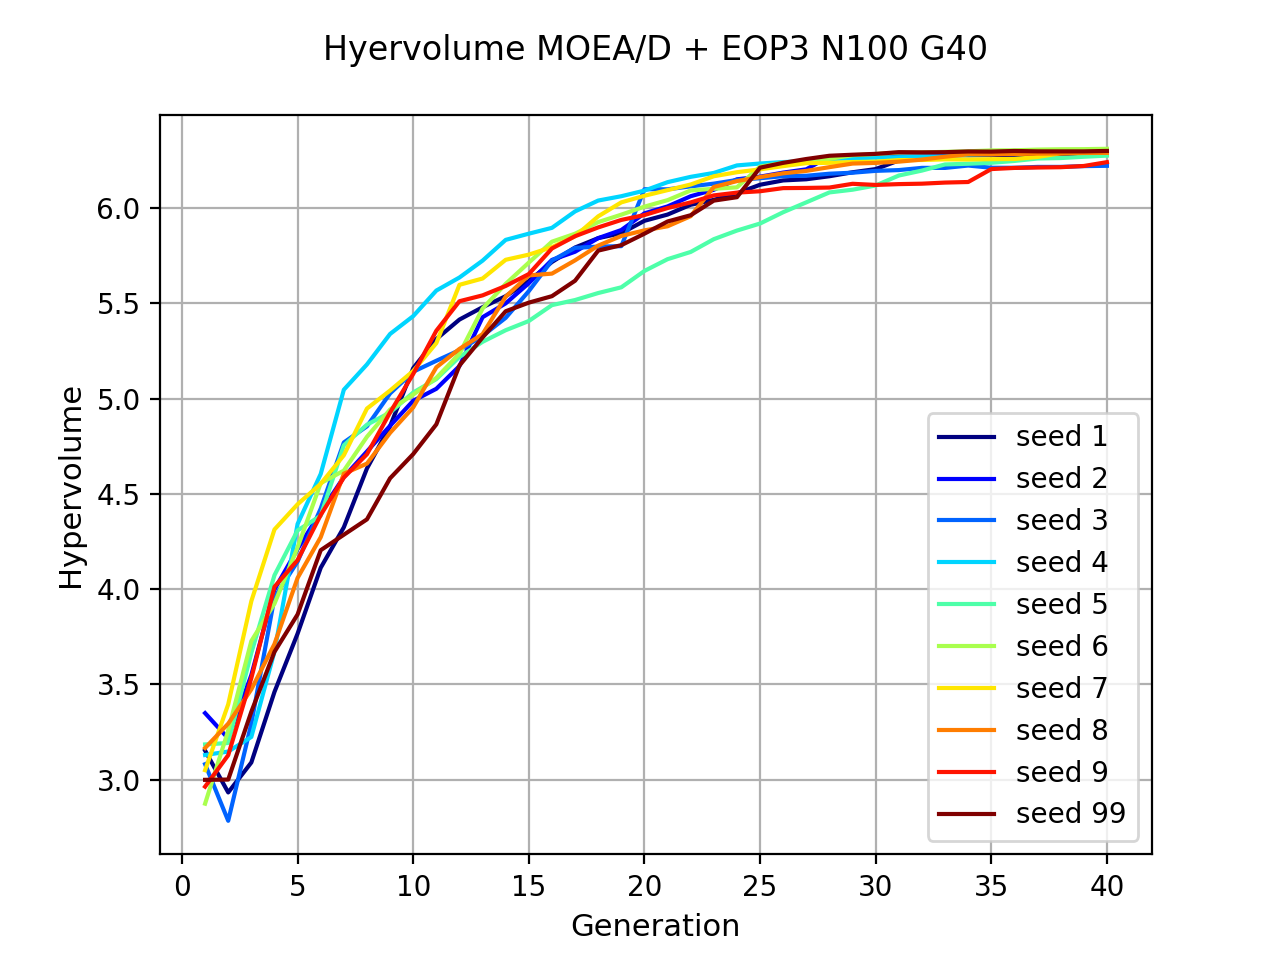
\includegraphics[scale=0.43]{figures/METRICS_EOP3/Hypervol_N100_G40.png}\quad 
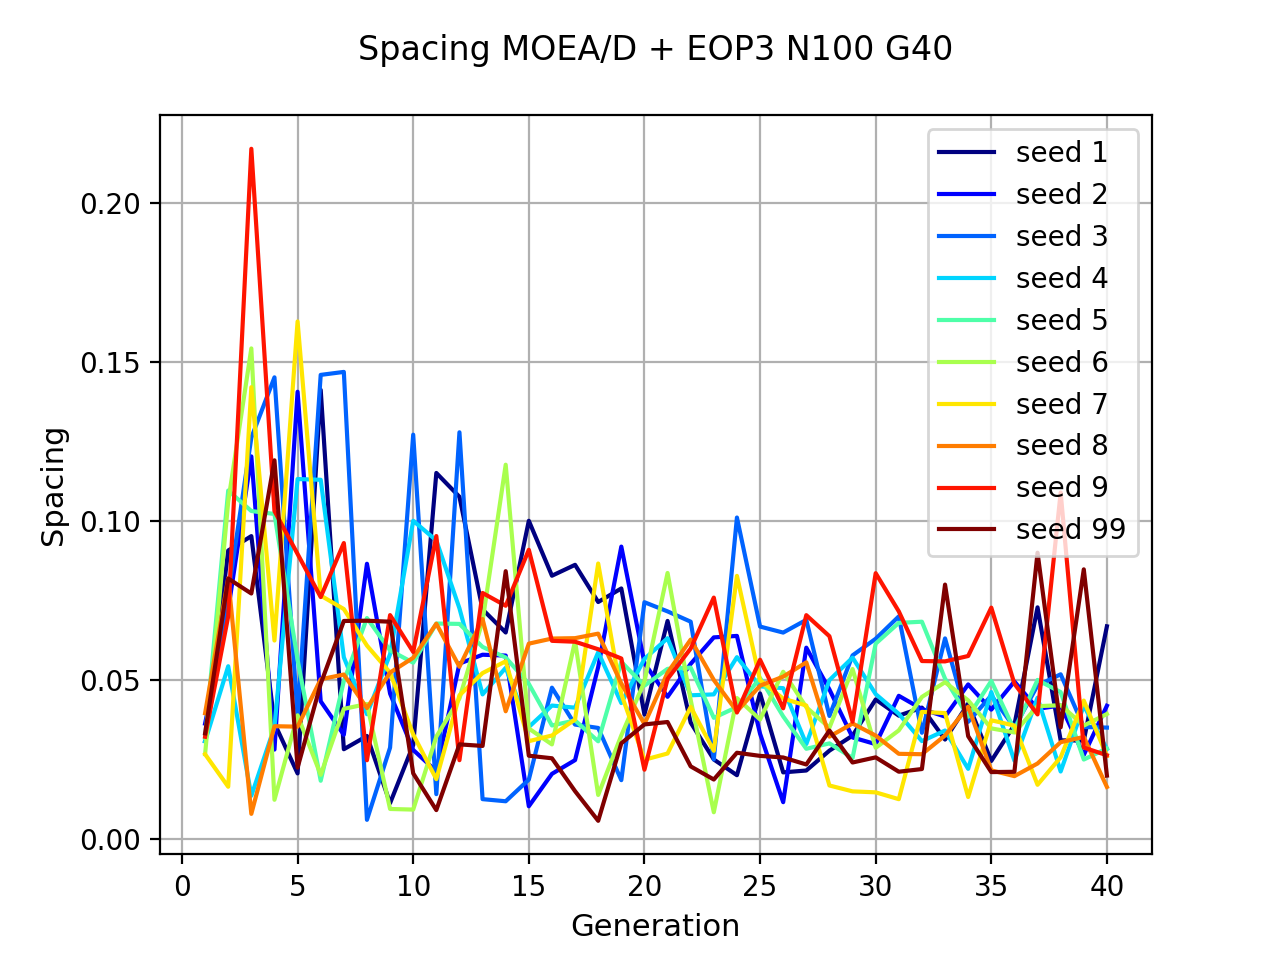
\includegraphics[scale=0.43]{figures/METRICS_EOP3/Spacing_N100_G40.png}\\
\caption{MOEA/D + EOP3. Métricas para 4000EV}
\label{fig:24}
\end{figure}


\begin{figure}[H]
\centering
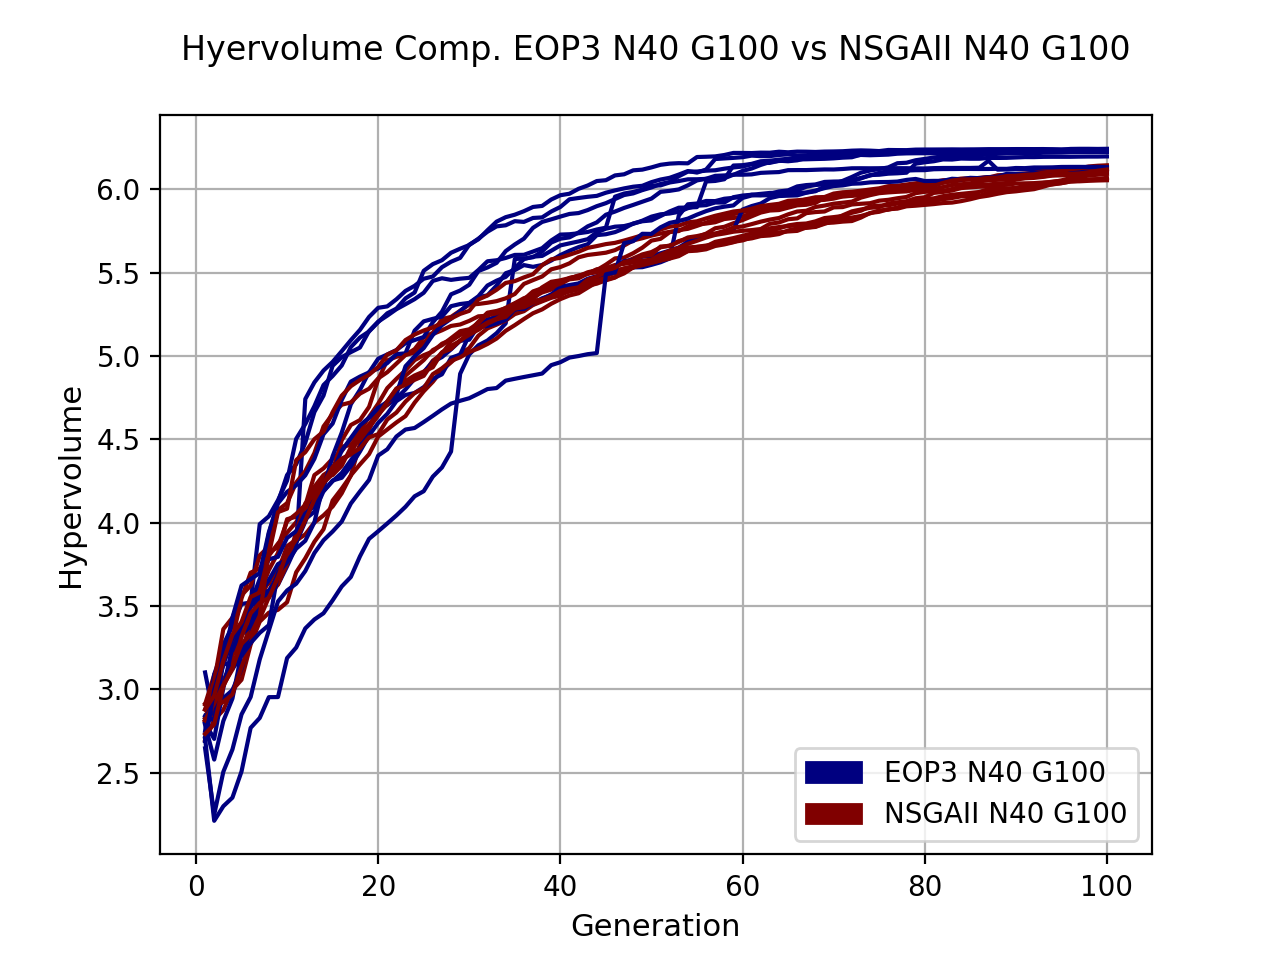
\includegraphics[scale=0.35]{../METRICS_PLOTS/Hypervol_COMP_EOP3N40G100_NSGAIIN40G100.png}
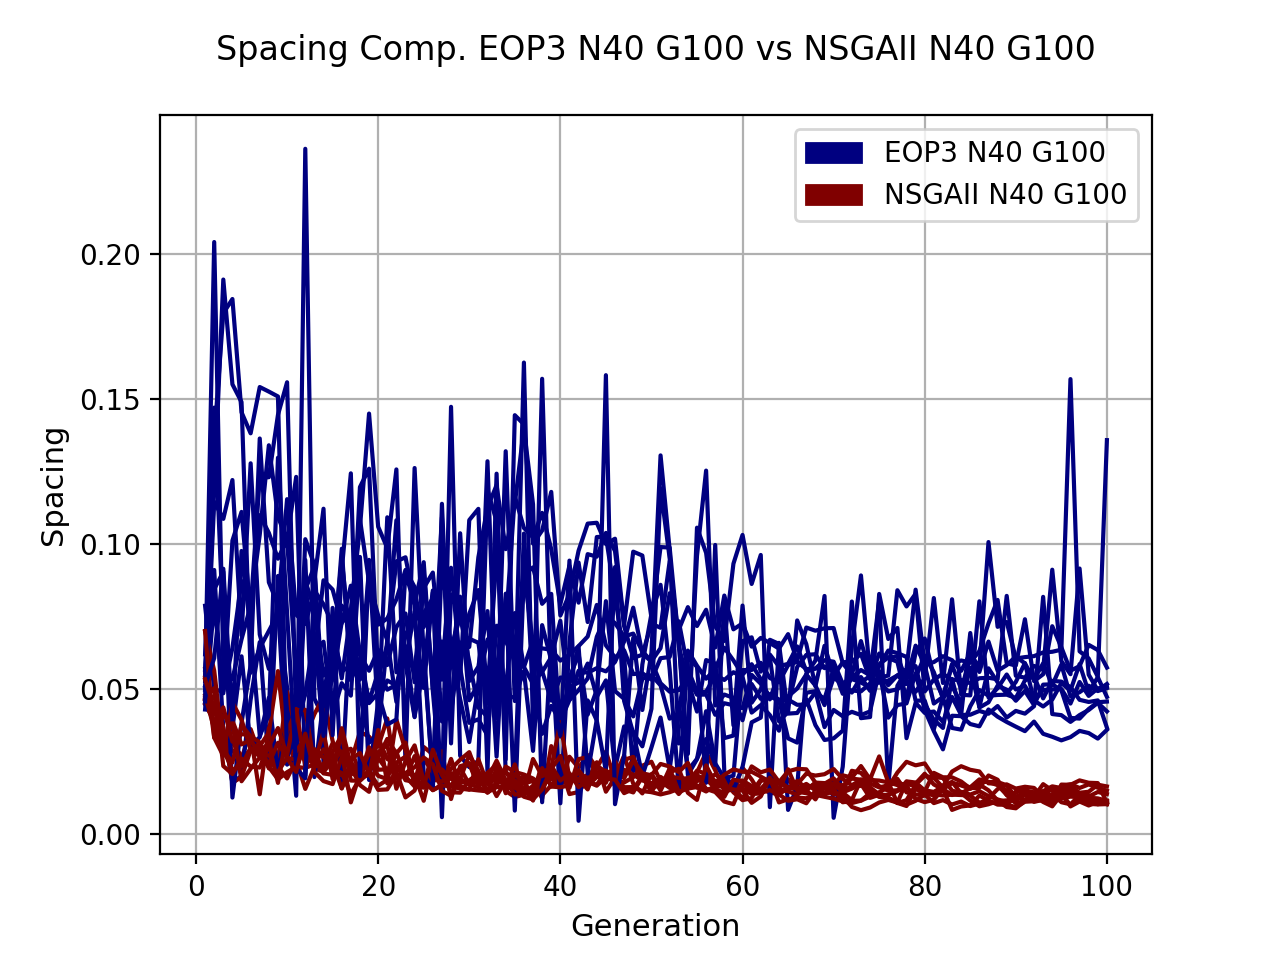
\includegraphics[scale=0.35]{../METRICS_PLOTS/Spacing_COMP_EOP3N40G100_NSGAIIN40G100.png}
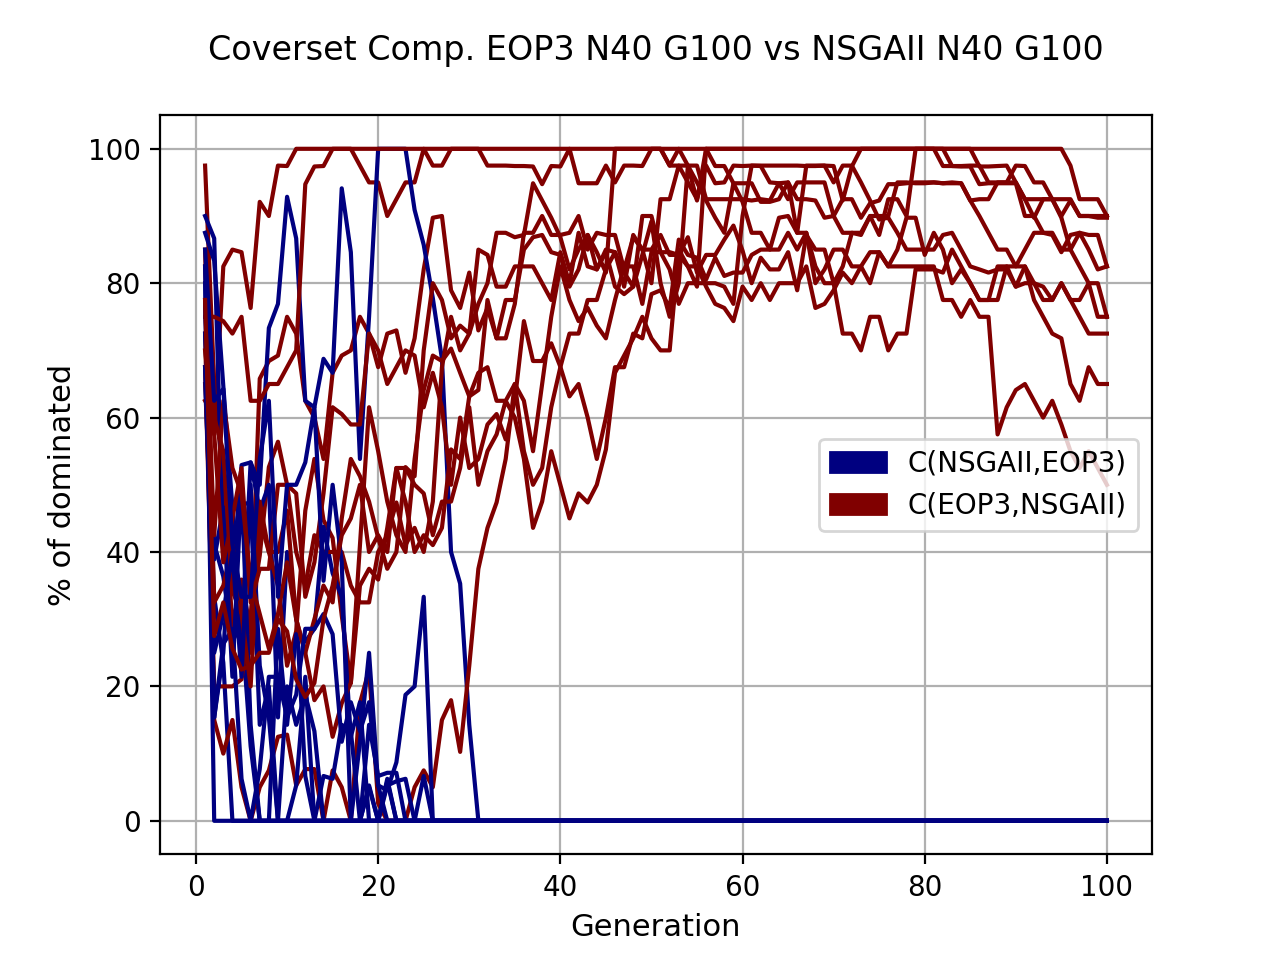
\includegraphics[scale=0.35]{../METRICS_PLOTS/CoverSet_COMP_EOP3N40G100_NSGAIIN40G100.png}\\
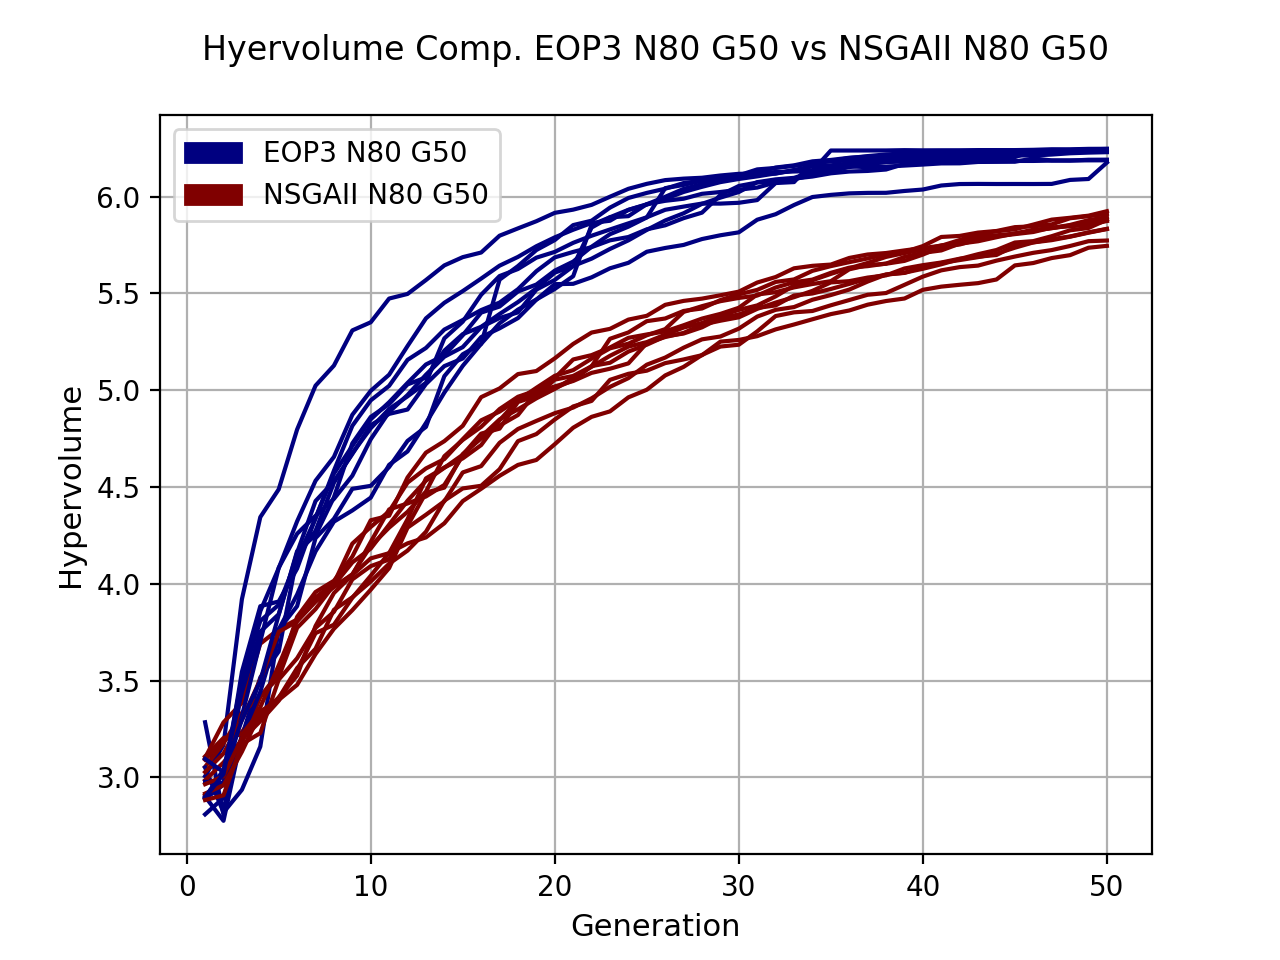
\includegraphics[scale=0.35]{../METRICS_PLOTS/Hypervol_COMP_EOP3N80G50_NSGAIIN80G50.png}
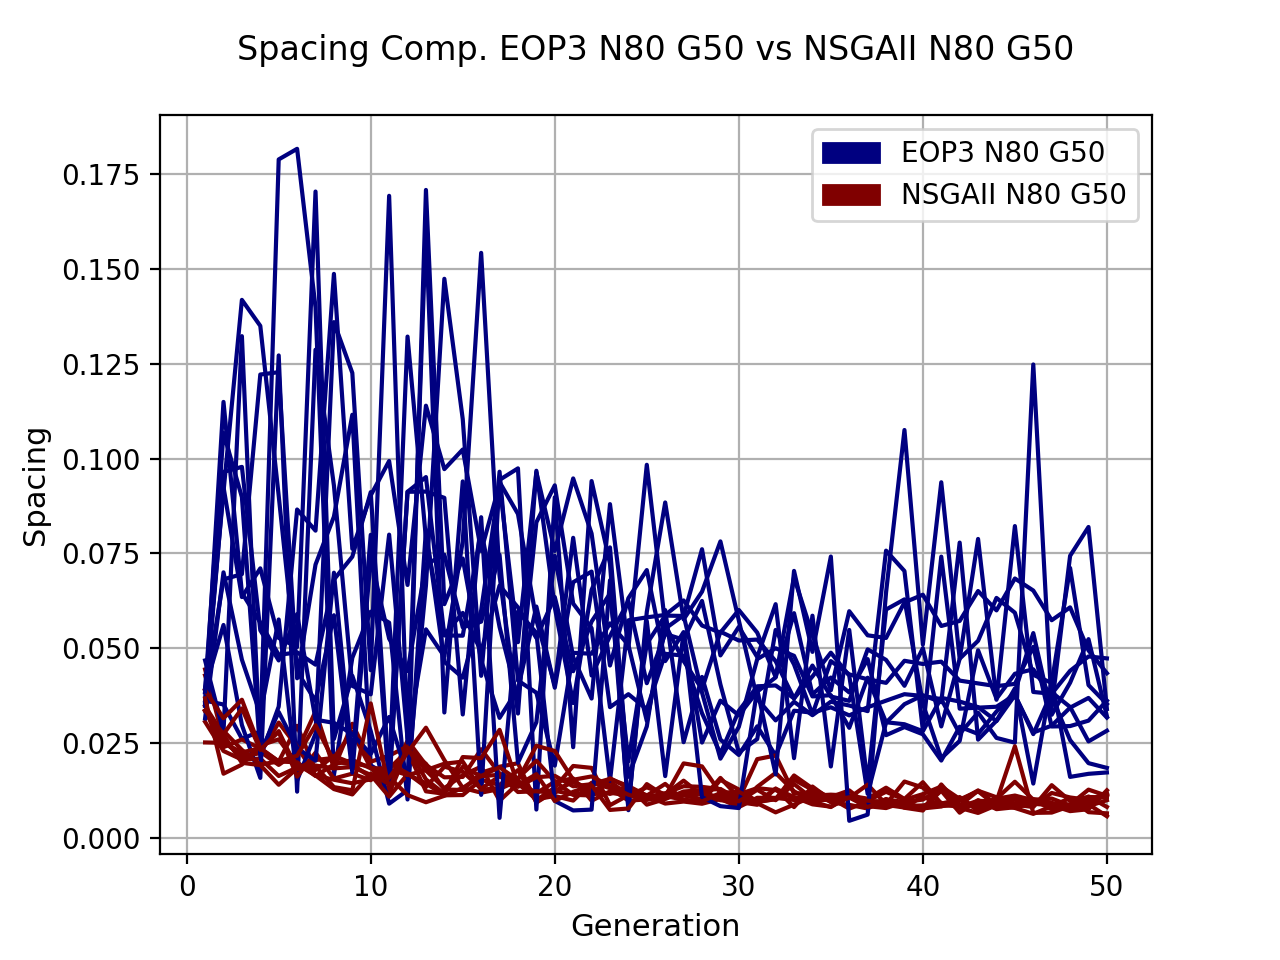
\includegraphics[scale=0.35]{../METRICS_PLOTS/Spacing_COMP_EOP3N80G50_NSGAIIN80G50.png}
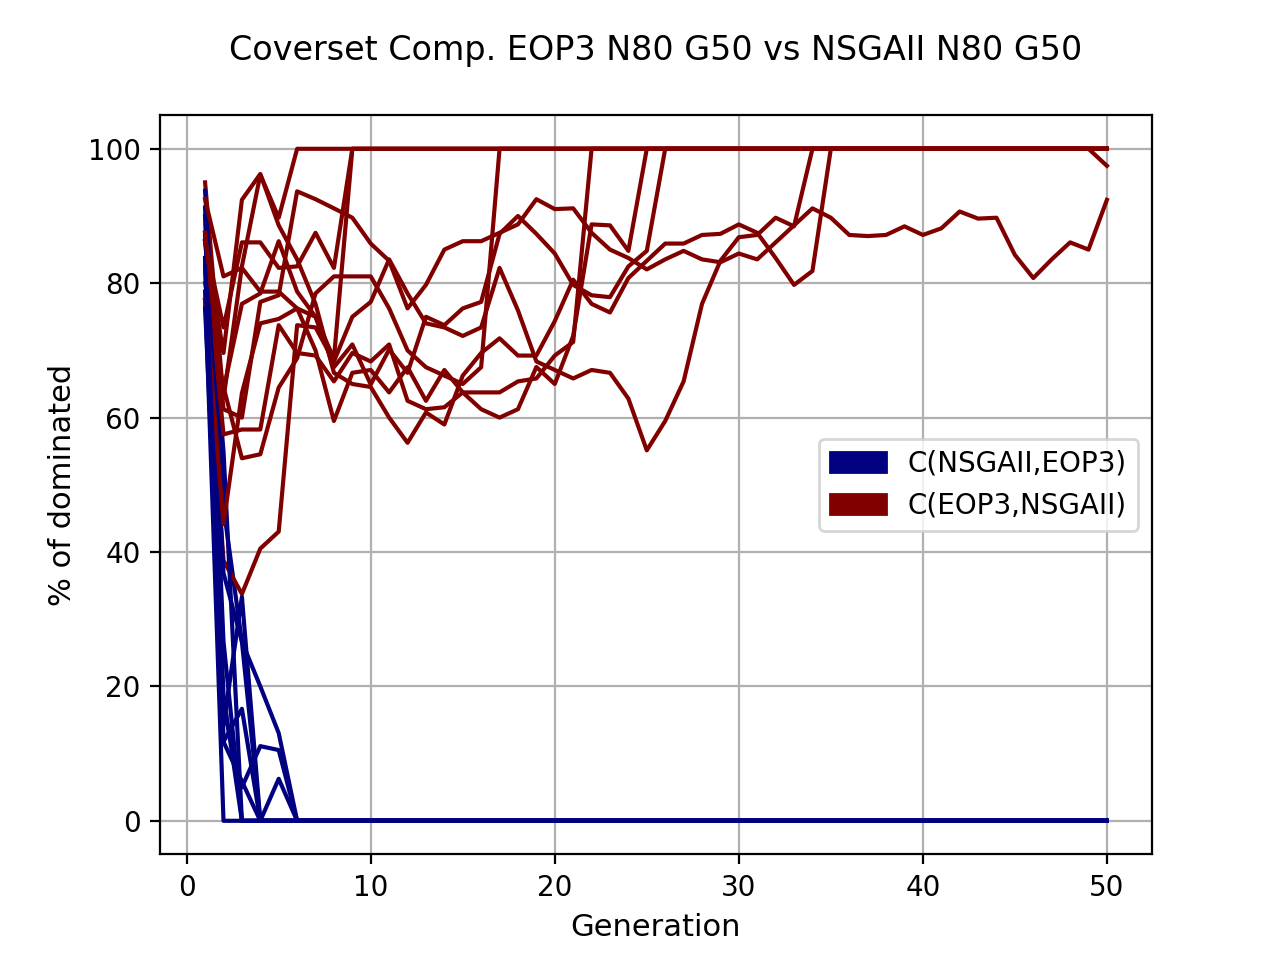
\includegraphics[scale=0.35]{../METRICS_PLOTS/CoverSet_COMP_EOP3N80G50_NSGAIIN80G50.png}\\
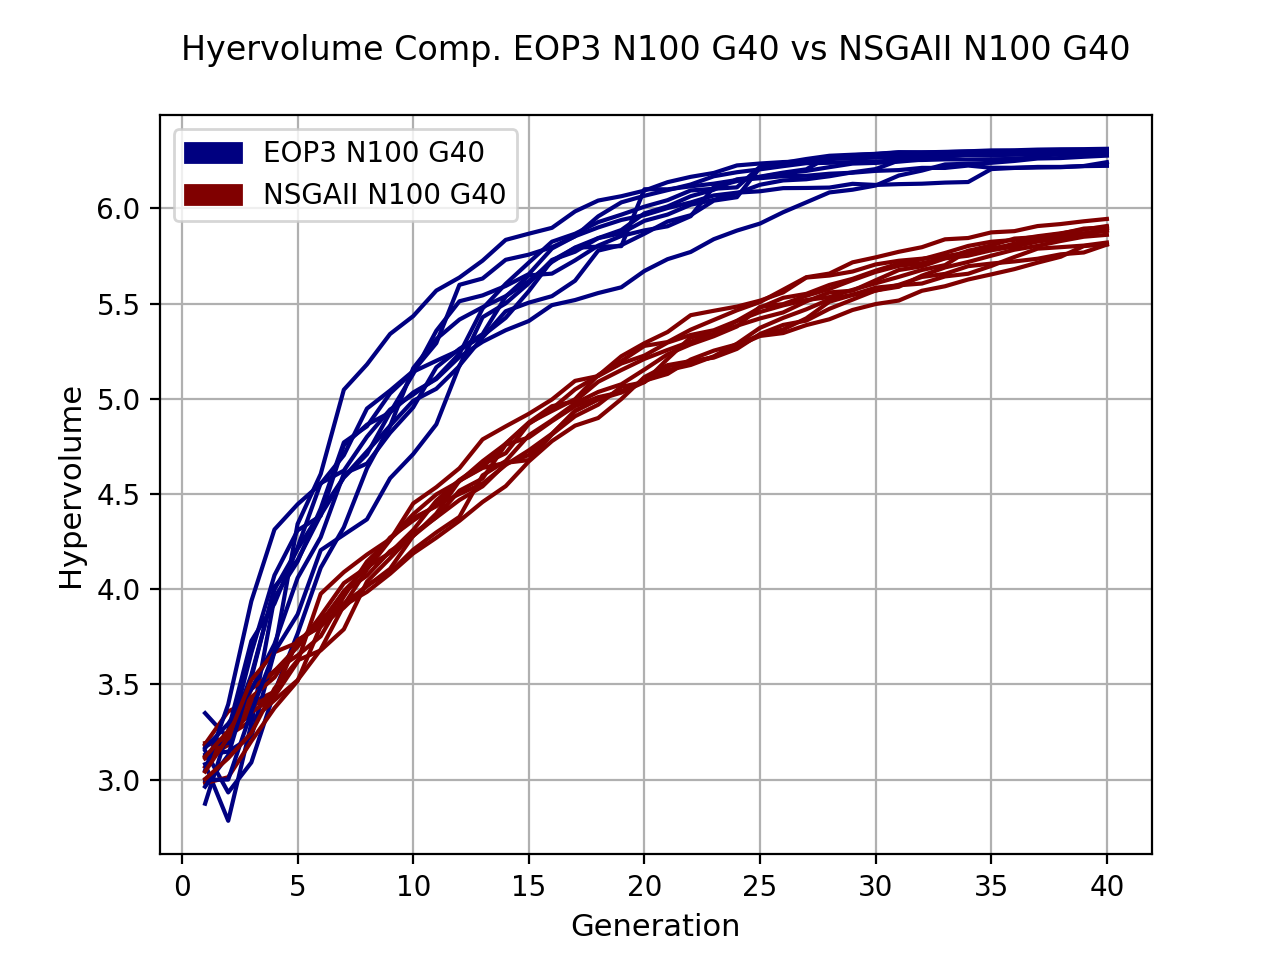
\includegraphics[scale=0.35]{../METRICS_PLOTS/Hypervol_COMP_EOP3N100G40_NSGAIIN100G40.png}
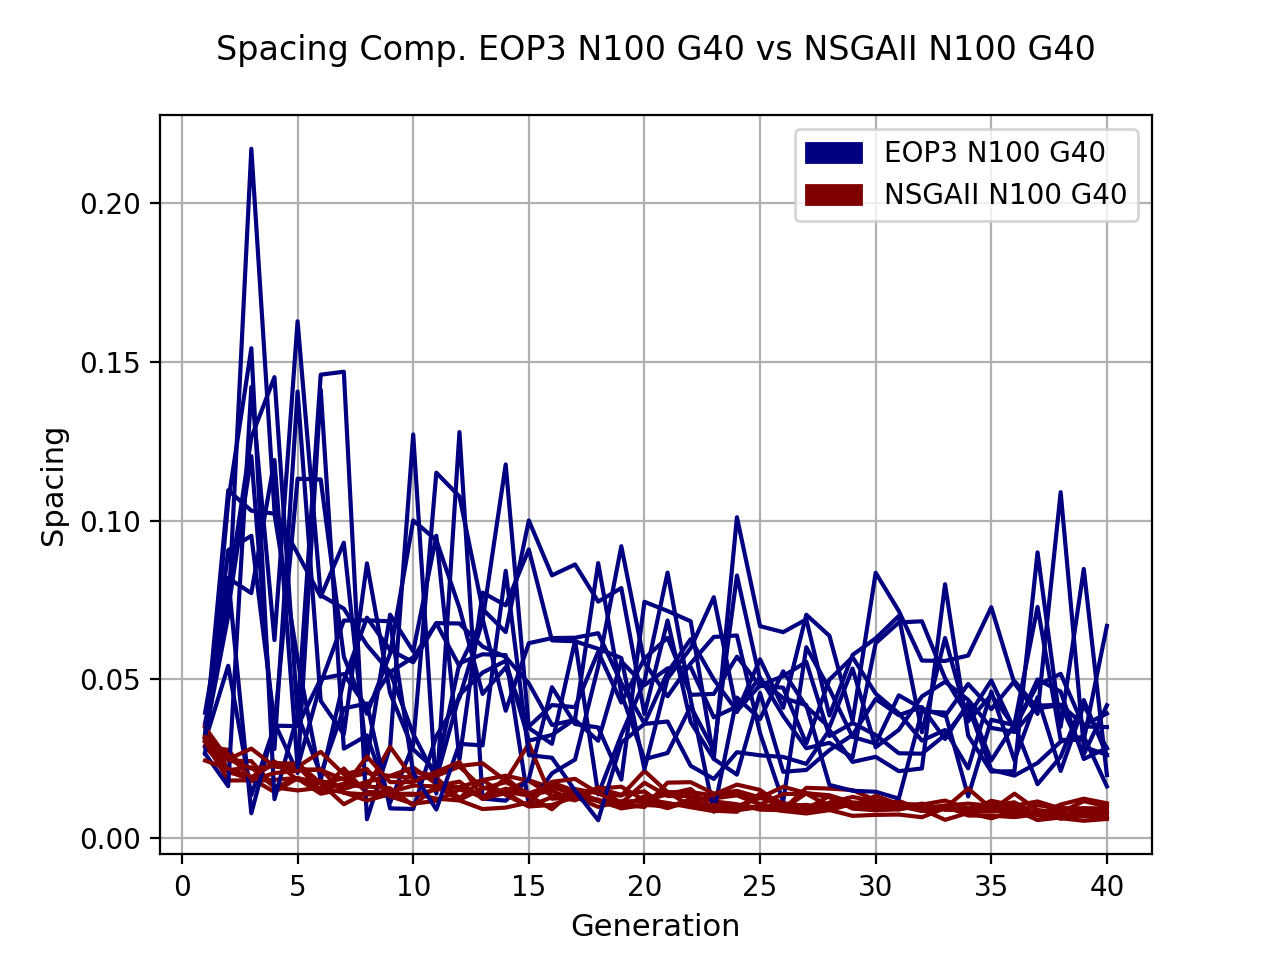
\includegraphics[scale=0.35]{../METRICS_PLOTS/Spacing_COMP_EOP3N100G40_NSGAIIN100G40.png}
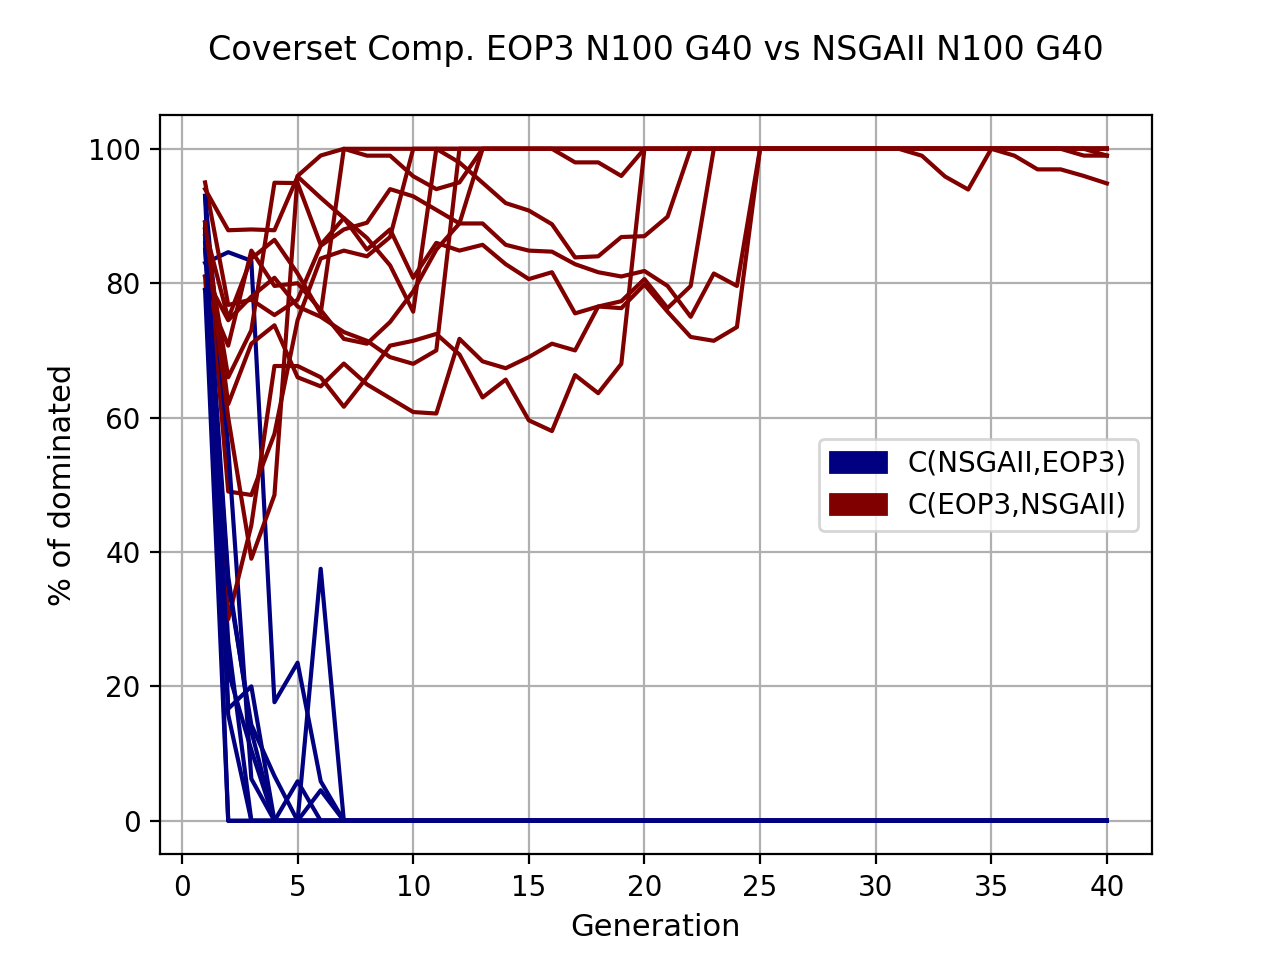
\includegraphics[scale=0.35]{../METRICS_PLOTS/CoverSet_COMP_EOP3N100G40_NSGAIIN100G40.png}\\
\caption{MOEA/D + EOP3. Comparación de métricas con NSGAII para 4000 EV.}
\label{fig:25}
\end{figure}